% =====================================================================
% DERCAS - PaTodo
% Documento de Especificaciones, Requerimientos y Criterios de
% Aceptacion de Software
% Compilacion: pdflatex main.tex  (dos veces para el indice)
% =====================================================================
\documentclass[12pt,a4paper]{article}

% --- Codificacion e idioma -----------------------------------------
\usepackage[utf8]{inputenc}
\usepackage[T1]{fontenc}
\usepackage[spanish,es-nodecimaldot]{babel}
\usepackage{lmodern}

% --- Pagina y margenes ---------------------------------------------
\usepackage[a4paper,left=3cm,right=2.5cm,top=3cm,bottom=2.5cm]{geometry}

% --- Paquetes de apoyo ---------------------------------------------
\usepackage{array}
\usepackage{longtable}
\usepackage{booktabs}
\usepackage{multirow}
\usepackage{tabularx}
\usepackage{float}
\usepackage{graphicx}
\usepackage{caption}
\usepackage{enumitem}
\usepackage{fancyhdr}
\usepackage{titlesec}
\usepackage{xcolor}
\usepackage{colortbl}
\usepackage{hyperref}
\usepackage{tikz}
\usetikzlibrary{
  positioning,
  arrows.meta,
  shapes.geometric,
  shapes.misc,
  calc,
  fit,
  backgrounds,
  chains,
  decorations.pathreplacing,
  automata,
  matrix,
  shadows
}
\tikzset{
  >=Latex,
  flowarrow/.style={-{Latex[length=2.5mm]},thick},
  decision/.style={diamond,draw,aspect=2,align=center,inner sep=1pt},
  process/.style={rectangle,draw,rounded corners,align=center,inner sep=4pt},
  startstop/.style={rectangle,draw,rounded corners=4pt,fill=gray!15,align=center,minimum width=22mm,inner sep=4pt},
  io/.style={trapezium,trapezium left angle=70,trapezium right angle=110,draw,align=center,inner sep=3pt},
  usecase/.style={ellipse,draw,fill=blue!8,align=center,minimum height=8mm,inner sep=2pt,font=\small},
  actor/.style={ellipse,draw,fill=orange!10,align=center,minimum height=9mm,minimum width=16mm,font=\small},
  entity/.style={rectangle,draw,align=center,font=\small\bfseries,inner sep=4pt},
  attr/.style={ellipse,draw,align=left,font=\scriptsize,inner sep=2pt}
}

% --- hyperref -------------------------------------------------------
\hypersetup{
  colorlinks=true,
  linkcolor=black,
  urlcolor=blue,
  pdftitle={DERCAS - PaTodo: Plataforma de servicios bajo demanda},
  pdfauthor={Equipo de Desarrollo PaTodo}
}

% --- Encabezado y pie ----------------------------------------------
\pagestyle{fancy}
\fancyhf{}
\setlength{\headheight}{14.6pt}
\fancyhead[L]{\small DERCAS -- PaTodo}
\fancyhead[R]{\small \leftmark}
\fancyfoot[C]{\thepage}
\renewcommand{\headrulewidth}{0.4pt}

% --- Títulos de sección --------------------------------------------
\titleformat{\section}{\normalfont\Large\bfseries}{\thesection}{0.6em}{}
\titleformat{\subsection}{\normalfont\large\bfseries}{\thesubsection}{0.6em}{}
\titleformat{\subsubsection}{\normalfont\normalsize\bfseries}{\thesubsubsection}{0.6em}{}

% --- Listas ---------------------------------------------------------
\setlist[itemize]{leftmargin=*,itemsep=2pt,topsep=3pt}
\setlist[enumerate]{leftmargin=*,itemsep=2pt,topsep=3pt}

% --- Entornos propios ----------------------------------------------
\newcolumntype{P}[1]{>{\raggedright\arraybackslash}p{#1}}
\newcolumntype{L}[1]{>{\raggedright\arraybackslash}p{#1}}
\setlength{\tabcolsep}{5pt}
\newenvironment{casos}{\small}{\normalsize}

\captionsetup[figure]{labelformat=empty}
\captionsetup{font=small}

% --- Página de título ----------------------------------------------
\begin{document}

\begin{titlepage}
\centering
\vspace*{1.5cm}

{\Large\bfseries SISTEMA DE GESTIÓN DE SERVICIOS BAJO DEMANDA\\[0.3em] PaTodo\par}

\vspace{1.2cm}

{\large Documento de Especificaciones, Requerimientos y Criterios de\\
Aceptación de Software --- DERCAS\par}

\vspace{0.8cm}

{\normalsize Departamento de Desarrollo de Sistemas\par}
\vspace{0.3cm}
{\normalsize PaTodo --- Servicios bajo demanda\par}

\vfill

\begin{tabular}{|P{4.2cm}|L{9.5cm}|}
\hline
\textbf{Proyecto} & PaTodo: plataforma que conecta clientes con trabajadores cercanos para la contratación de servicios generales, del hogar y de emergencias. \\ \hline
\textbf{Versión del documento} & 1.0 \\ \hline
\textbf{Fecha} & Octubre de 2026 \\ \hline
\textbf{Estado} & En producción (API REST, frontend web y reglas de seguridad desplegadas) \\ \hline
\textbf{Elaborado por} & Equipo de Desarrollo de Sistemas --- PaTodo \\ \hline
\textbf{Fuente de verdad} & \texttt{spec/openapi.yaml} y \texttt{spec/schemas/} (Especificación OpenAPI 3 y JSON Schemas) \\ \hline
\end{tabular}

\vfill
\end{titlepage}

% --- Índice ---------------------------------------------------------
\tableofcontents
\newpage

% =====================================================================
% 1. DEFINICIONES, ACRÓNIMOS Y ABREVIATURAS
% =====================================================================
\section{Definiciones, acrónimos y abreviaturas}

\begin{longtable}{|P{3.3cm}|L{11.2cm}|}
\hline
\textbf{Término} & \textbf{Concepto} \\ \hline
\endfirsthead
\hline
\textbf{Término} & \textbf{Concepto} \\ \hline
\endhead
\hline
\endfoot

API & Interfaz de programación de aplicaciones. Pieza de código que permite que dos aplicaciones se comuniquen entre sí y compartan información y funcionalidades; es el intermediario que permite que un sistema pida datos o ejecute acciones específicas. En PaTodo la implementa el servicio REST en Express, desplegado en Render. \\ \hline

Backend & Arquitectura interna de una aplicación, no visible para el usuario. Se encarga de la lógica de negocio, de recibir peticiones y devolver datos procesados. En PaTodo lo componen los servicios gestionados de Firebase y la API REST transaccional. \\ \hline

Browser & Navegador web o explorador de Internet. \\ \hline

Casos de uso & Descripción de una acción o actividad. El diagrama de casos de uso describe las actividades que debe realizar alguien o algo para llevar a cabo un proceso dentro del sistema. \\ \hline

Client (SDK) & Bibliotecas oficiales de Firebase para el cliente (Web y móvil) que permiten autenticación, lectura en tiempo real y escritura directa sobre documentos propios del usuario, siempre validadas por las reglas de seguridad. \\ \hline

CORS & \textit{Cross-Origin Resource Sharing}. Mecanismo que permite que un navegador acepte peticiones desde orígenes distintos al que sirve la aplicación; en PaTodo se restringe mediante una lista blanca en la variable \texttt{CORS\_ORIGINS}. \\ \hline

CRUD & Siglas de \textit{Crear, Leer, Actualizar y Eliminar}; las cuatro operaciones básicas sobre los datos de una aplicación. \\ \hline

Custom Claim & Declaración personalizada que viaja dentro del ID token de Firebase Authentication. PaTodo la usa para transportar el rol (\texttt{role}) hasta las reglas de seguridad de Firestore. \\ \hline

DERCAS & \textit{Documento de Especificaciones, Requerimientos y Criterios de Aceptación de Software}. Documento que describe el sistema solicitado, sus actores, procesos, casos de uso, requisitos y criterios de aceptación. \\ \hline

Docker & Herramienta que automatiza el despliegue de aplicaciones, permitiendo crear, probar e implementar de forma reproducible. \\ \hline

FCM & \textit{Firebase Cloud Messaging}. Servicio de notificaciones push que entrega avisos a los dispositivos de los usuarios; en PaTodo lo usa la API REST mediante el Admin SDK. \\ \hline

Firestore & Base de datos de documentos de Google Firebase, con escalado automático, consultas en tiempo real y reglas de seguridad declarativas. Es el almacén de datos de PaTodo. \\ \hline

Frontend & Parte de una aplicación que interactúa con los usuarios; es el lado del cliente, es decir, lo que se ve en pantalla. En PaTodo existe una versión web (React) y una móvil (Flutter). \\ \hline

GeoPoint / Geohash & Tipo de dato de Google para representar coordenadas geográficas y, respectivamente, su codificación de cadena corta. PaTodo almacena el \texttt{geohash} dentro del \texttt{location} de los usuarios y los trabajos para habilitar búsquedas por proximidad. \\ \hline

Geofire (geofire-common) & Librería que calcula el \texttt{geohash} de un \texttt{GeoPoint} y los límites del área (\texttt{geohashQueryBounds}) que la cubre, base de la búsqueda de trabajos cercanos. \\ \hline

Haversine & Fórmula trigonométrica para calcular la distancia en línea recta entre dos coordenadas geográficas. PaTodo la usa para descartar los trabajos que caen fuera del radio solicitado. \\ \hline

HTTPS & Protocolo de transferencia de hipertexto seguro; destino cifrado de las comunicaciones. \\ \hline

ID Token & Token de identidad que emite Firebase Authentication tras iniciar sesión. PaTodo lo envía el cliente en la cabecera \texttt{Authorization: Bearer} y la API lo verifica con el Admin SDK. \\ \hline

OpenAPI 3 & Especificación estándar (YAML) que describe de forma formal las operaciones HTTP de una API: rutas, parámetros, esquemas de entrada y respuestas. En PaTodo vive en \texttt{spec/openapi.yaml} y es la fuente única de verdad de los contratos. \\ \hline

OSRM & \textit{Open Source Routing Machine}. Motor de cálculo de rutas por carretera. PaTodo lo consulta la API REST para obtener la geometría, la distancia y la duración del trayecto. \\ \hline

Patrón MVC & \textit{Modelo-Vista-Controlador}. Separación del software en modelo (datos), vista (interfaz) y controlador (lógica). \\ \hline

PWA / SPA & \textit{Progressive Web Application} / \textit{Single Page Application}: aplicación web que ejecuta su contenido en una sola página, sin recargas completas. \\ \hline

REST & Interfaz para conectar sistemas sobre HTTP; obtiene y genera datos devolviéndolos en formatos definidos, como JSON. \\ \hline

SDK & \textit{Software Development Kit} (kit de desarrollo de software). \\ \hline

Spec-Driven Development (SDD) & Metodología adoptada en PaTodo: primero se define el contrato en la especificación (\texttt{spec/}) y después se implementa en la API y en los frontends. \\ \hline

SSO & \textit{Single Sign-On} (inicio de sesión único): procedimiento que habilita a un usuario para acceder a varios sistemas con una sola autenticación. \\ \hline

TURN / STUN & Servidores de apoyo del trayecto de una conexión WebRTC: STUN descubre la dirección pública del dispositivo y TURN la retransmite cuando la conexión directa no es posible (por ejemplo, detrás de CGNAT). \\ \hline

WebRTC & Tecnología de navegador que permite comunicación de voz y video en tiempo real entre dos puntos (peer-to-peer), sin pasar por un servicio de transmisión central. \\ \hline

XLSX / PDF & Formatos de hoja de cálculo y de documento portátil, respectivamente. \\ \hline
\end{longtable}

% =====================================================================
% 2. DESCRIPCIÓN DEL SISTEMA SOLICITADO
% =====================================================================
\section{Descripción del sistema solicitado}

En la actualidad, la contratación de servicios generales, del hogar y de emergencia (mecánica, plomería, jardinería, pintura, instalación eléctrica, etc.) depende de contactos informales, llamadas telefónicas o anuncios aislados, lo que dificulta encontrar un profesional disponible cerca de la ubicación del cliente, comparar precios y evaluar la calidad del trabajo realizado.

Se solicita el desarrollo e implementación de una plataforma de servicios bajo demanda, denominada \textbf{PaTodo}, que conecte clientes con trabajadores independientes cercanos, permitiendo que el cliente publique un trabajo, que los trabajadores cercanos lo descubran y envíen ofertas, y que el cliente elija la mejor opción. El sistema debe permitir:

\begin{itemize}
    \item El registro y la autenticación de clientes y trabajadores, con una plataforma web y una aplicación móvil.
    \item La publicación de trabajos, especificando descripción, categoría, habilidades requeridas, ubicación (recogida y destino opcional), precio propuesto y fecha programada.
    \item La búsqueda de trabajos cercanos al trabajador por proximidad geográfica, con filtros de categoría y radio de búsqueda.
    \item El envío de ofertas por parte de los trabajadores, con precio, tiempo estimado y mensaje, sobre trabajos ajenos y en estado pendiente.
    \item La aceptación de una oferta por parte del cliente, lo que asigna al trabajador seleccionado y abre automáticamente una conversación privada.
    \item La cancelación del trabajo por parte del cliente mientras no haya sido completado.
    \item El seguimiento de la ubicación del trabajador en tiempo real y el cálculo de la ruta entre los puntos del trayecto.
    \item La finalización del trabajo y la calificación mutua entre cliente y trabajador, con puntuación y comentario.
    \item Las notificaciones en tiempo real de los eventos relevantes (nuevas ofertas, aceptación, finalización, calificación).
    \item La comunicación de voz entre las partes del trabajo mediante conexión WebRTC punto a punto, con señalización persistida en la base de datos.
    \item Un módulo de administración para la gestión de usuarios, verificación de profesionales, suspensión y activación de cuentas, promoción de administradores y mantenimiento del catálogo de categorías y habilidades.
\end{itemize}

El sistema se construirá sobre una arquitectura de servicios gestionados en la nube: autenticación, base de datos de documentos, notificaciones push y almacenamiento en Firebase, más una API REST transaccional propia en Node.js/Express responsable de las operaciones atómicas. Las interfaces de usuario se comunican con estos servicios mediante los SDK oficiales y la API REST.

El desarrollo se apoya, además, en un modelo de desarrollo orientado a especificaciones (\textit{Spec-Driven Development}), de modo que los contratos de datos y de API se documentan formalmente antes de implementarse y constituyen la fuente única de verdad del proyecto.

% =====================================================================
% 3. DEFINICIÓN DE ACTORES
% =====================================================================
\section{Definición de actores}

\begin{longtable}{|P{3.3cm}|L{11.2cm}|}
\hline
\textbf{Nombre del actor} & \textbf{Descripción} \\ \hline
\endfirsthead
\hline
\textbf{Nombre del actor} & \textbf{Descripción} \\ \hline
\endhead
\hline
\endfoot



Cliente (\texttt{client}) & Usuario que contrata servicios. Publica trabajos, revisa las ofertas recibidas, acepta la oferta que mejor le convenga, cancela trabajos no finalizados, conversa con el trabajador asignado, sigue su ubicación, finaliza el trabajo y califica al profesional. \\ \hline

Trabajador (\texttt{worker}) & Usuario que ofrece servicios. Consulta los trabajos cercanos a su ubicación mediante búsqueda geográfica, calcula la ruta hacia el trabajo, envía ofertas, gestiona sus propias ofertas (editar o retirar), reporta su ubicación durante el trayecto, finaliza el trabajo y califica al cliente. \\ \hline

Ambos (\texttt{both}) & Usuario que puede actuar indistintamente como cliente y como trabajador. La aplicación le habilita ambos conjuntos de acciones según el contexto de la pantalla. \\ \hline

Administrador (\texttt{admin}) & Superusuario del sistema. Accede al panel de administración para consultar métricas de operación, listar y filtrar usuarios y trabajos, cambiar roles, promover o revocar administradores, suspender o activar cuentas, verificar profesionales y mantener el catálogo de categorías y habilidades. \\ \hline

API REST (actor interno) & Componente de servidor que actúa como actor del sistema. Verifica el ID token de cada petición, ejecuta las transacciones que exigen atomicidad (aceptar oferta, cancelar, completar, calcular ruta, crear reseña, sesión de voz) y genera las notificaciones correspondientes. \\ \hline

Reglas de seguridad de Firestore (actor interno) & Componente que autoriza las escrituras directas de los clientes a partir del rol declarado en el token y de la propiedad del recurso. \\ \hline

\end{longtable}

% =====================================================================
% 4. PROCESOS A SISTEMATIZAR
% =====================================================================
\section{Procesos a sistematizar}

A continuación se describen los procesos de negocio que el sistema debe automatizar. Cada proceso indica su descripción, los actores involucrados, sus entradas y salidas, las especificaciones de funcionamiento y las restricciones adicionales que condicionan su implementación.

% ---------------------------------------------------------------------
\subsection{Autenticación y gestión de cuentas}

\begin{longtable}{|P{3.3cm}|L{11.2cm}|}
\hline
\textbf{Nombre} & Autenticación y gestión de cuentas \\ \hline
\textbf{Descripción} & Registro e inicio de sesión de clientes y trabajadores mediante correo electrónico y contraseña, así como mediante Google Sign-In. Una vez autenticado, el usuario completa su perfil (nombre, teléfono, foto de perfil) y selecciona el rol con el que operar (\texttt{client}, \texttt{worker} o \texttt{both}), lo que genera el documento \texttt{users/\{uid\}} y asigna el Custom Claim \texttt{role}. \\ \hline
\textbf{Actores} & Cliente, Trabajador, API REST \\ \hline
\textbf{Entradas} & Correo electrónico, contraseña, o credenciales de Google; nombre, teléfono y rol seleccionado. \\ \hline
\textbf{Salidas} & Sesión iniciada con ID token; documento de usuario creado; Custom Claim \texttt{role} asignado. \\ \hline
\textbf{Especificaciones de funcionamiento} & El registro y el inicio de sesión se resuelven directamente contra Firebase Authentication desde el cliente. La creación del perfil se realiza mediante \texttt{POST /createUser}, que valida que el \texttt{uid} y el correo coincidan con los del token, crea el documento de usuario y asigna el rol como \textit{Custom Claim}. Al finalizar, el cliente debe refrescar su ID token (\texttt{getIdToken(true)}) para que el rol viaje en las peticiones. Los usuarios previos a la asignación del rol se actualizan con la utilidad de sincronización de claims. \\ \hline
\textbf{Restricciones adicionales} & Un usuario no puede publicar trabajos con el rol \texttt{worker} ni enviar ofertas con el rol \texttt{client}. No puede crearse un segundo perfil para el mismo \texttt{uid}. El teléfono es obligatorio para completar el perfil. \\ \hline
\end{longtable}

% ---------------------------------------------------------------------
\subsection{Configuración del catálogo de servicios}

\begin{longtable}{|P{3.3cm}|L{11.2cm}|}
\hline
\textbf{Nombre} & Configuración del catálogo de servicios \\ \hline
\textbf{Descripción} & Administración de las colecciones maestras \texttt{categories} y \texttt{skills}, que sustentan la clasificación de los trabajos publicados. Cada habilidad se asocia a una o más categorías mediante \texttt{categoryIds}. \\ \hline
\textbf{Actores} & Administrador \\ \hline
\textbf{Entradas} & Datos de la categoría (código, nombre, descripción, icono, color, imagen, orden, estado activo) y de la habilidad (código, nombre, categorías asociadas, estado activo). \\ \hline
\textbf{Salidas} & Catálogos actualizados, disponibles para los formularios de publicación de trabajos y para los filtros de búsqueda. \\ \hline
\textbf{Especificaciones de funcionamiento} & La lectura de ambos catálogos es pública, incluso sin autenticar. La creación, actualización y eliminación está reservada al rol \texttt{admin}, tanto en las reglas de seguridad como en el panel web. El despliegue inicial se realiza con el catálogo semilla (8 categorías y 12 habilidades), una operación no destructiva que realiza \textit{upsert} con identificadores deterministas iguales al \texttt{slug} del elemento. \\ \hline
\textbf{Restricciones adicionales} & Un cliente o trabajador nunca puede modificar el catálogo. La operación de siembra de pruebas que borra la base de datos está prohibida en producción. \\ \hline
\end{longtable}

% ---------------------------------------------------------------------
\subsection{Publicación de trabajos}

\begin{longtable}{|P{3.3cm}|L{11.2cm}|}
\hline
\textbf{Nombre} & Publicación de trabajos \\ \hline
\textbf{Descripción} & El cliente publica una solicitud de servicio indicando en qué necesita ayuda, en qué categoría, qué habilidades se requieren, dónde se prestará el servicio (lugar de recogida), si hay un punto de entrega, cuánto está dispuesto a pagar y, opcionalmente, la fecha en que se requiere. \\ \hline
\textbf{Actores} & Cliente, Trabajador (destinatario), API REST (notificación) \\ \hline
\textbf{Entradas} & Descripción del trabajo, \texttt{categoryId}, \texttt{skillIds}, ubicación con coordenadas y \texttt{geohash}, precio propuesto, destino opcional, fecha programada opcional. \\ \hline
\textbf{Salidas} & Documento \texttt{jobs/\{id\}} en estado \texttt{pending}, visible en la búsqueda de trabajos cercanos. \\ \hline
\textbf{Especificaciones de funcionamiento} & La publicación se realiza con escritura directa del cliente sobre Firestore. La regla de seguridad exige rol \texttt{client} o \texttt{both}, que la cuenta no esté suspendida, que \texttt{clientId} coincida con el \texttt{uid} del token y que el trabajo nazca en estado \texttt{pending}. El cliente puede editar únicamente \texttt{details}, \texttt{pricing}, \texttt{location} y \texttt{updatedAt}, y puede eliminar el trabajo únicamente mientras siga en estado \texttt{pending}; cualquier otro cambio de estado se realiza exclusivamente a través de la API. \\ \hline
\textbf{Restricciones adicionales} & El cliente no puede asignar \texttt{workerId}, \texttt{acceptedOfferId}, \texttt{status} ni \texttt{route} por escritura directa; hacerlo le permitiría auto-completar el trabajo y fabricar reseñas. \\ \hline
\end{longtable}

% ---------------------------------------------------------------------
\subsection{Búsqueda de trabajos cercanos y notificación}

\begin{longtable}{|P{3.3cm}|L{11.2cm}|}
\hline
\textbf{Nombre} & Búsqueda de trabajos cercanos y notificación \\ \hline
\textbf{Descripción} & El trabajador consulta los trabajos pendientes próximos a su ubicación, filtrados por radio de búsqueda y, opcionalmente, por categoría. \\ \hline
\textbf{Actores} & Trabajador, API REST \\ \hline
\textbf{Entradas} & Latitud, longitud, radio en kilómetros (por defecto 10, máximo 50), categoría opcional y límite de resultados (por defecto 20, máximo 50). \\ \hline
\textbf{Salidas} & Listado de trabajos con la distancia en línea recta expresada en kilómetros, ordenada de menor a mayor. \\ \hline
\textbf{Especificaciones de funcionamiento} & La búsqueda se realiza mediante \texttt{GET /jobs/nearby}. El servicio calcula los límites geográficos del radio solicitado, consulta los trabajos en estado \texttt{pending} cuyo \texttt{location.geohash} cae dentro de esos límites mediante el índice compuesto de la base de datos y descarta los que superen el radio tras aplicar la fórmula de Haversine. La distancia mostrada es en línea recta y \textbf{no} representa la ruta por carretera. \\ \hline
\textbf{Restricciones adicionales} & Solo los roles \texttt{worker} y \texttt{both} pueden consultar; un cliente recibe \texttt{403}. Un trabajo sin \texttt{location.geohash} publicado no aparece en los resultados. Los parámetros con formato inválido o fuera de rango se rechazan con \texttt{400}. \\ \hline
\end{longtable}

% ---------------------------------------------------------------------
\subsection{Envío y gestión de ofertas}

\begin{longtable}{|P{3.3cm}|L{11.2cm}|}
\hline
\textbf{Nombre} & Envío y gestión de ofertas \\ \hline
\textbf{Descripción} & El trabajador envía una oferta económica y operativa para un trabajo cercano: precio propuesto, tiempo estimado de ejecución y mensaje para el cliente. \\ \hline
\textbf{Actores} & Trabajador, Cliente \\ \hline
\textbf{Entradas} & \texttt{jobId}, precio, tiempo estimado, moneda, mensaje. \\ \hline
\textbf{Salidas} & Documento \texttt{offers/\{id\}} en estado \texttt{pending}, visible para el cliente dueño del trabajo. \\ \hline
\textbf{Especificaciones de funcionamiento} & El envío se realiza con escritura directa del cliente. La regla exige rol \texttt{worker} o \texttt{both}, que \texttt{workerId} coincida con el \texttt{uid} del token, que la oferta nazca en estado \texttt{pending} y que el trabajo referenciado esté en estado \texttt{pending} y \textbf{no pertenezca al propio trabajador}. El trabajador puede editar precio, mensaje, tiempo estimado, moneda y estado de su propia oferta; el único cambio de estado permitido por escritura directa es de \texttt{pending} a \texttt{withdrawn}. \\ \hline
\textbf{Restricciones adicionales} & Un trabajador no puede ofertar por su propio trabajo. No puede modificar el \texttt{jobId} ni el \texttt{workerId}, ni auto-aceptar su oferta. Las ofertas no se borran: se retiran mediante el estado \texttt{withdrawn}. \\ \hline
\end{longtable}

% ---------------------------------------------------------------------
\subsection{Aceptación de oferta y asignación}

\begin{longtable}{|P{3.3cm}|L{11.2cm}|}
\hline
\textbf{Nombre} & Aceptación de oferta y asignación \\ \hline
\textbf{Descripción} & El cliente selecciona, entre las ofertas recibidas, la que mejor le conviene según precio, tiempo estimado, perfil y calificación del trabajador. \\ \hline
\textbf{Actores} & Cliente, API REST \\ \hline
\textbf{Entradas} & \texttt{jobId}, \texttt{offerId}. \\ \hline
\textbf{Salidas} & Trabajo en estado \texttt{accepted} con el trabajador asignado; resto de ofertas en \texttt{rejected}; conversación privada creada; notificación push a las partes. \\ \hline
\textbf{Especificaciones de funcionamiento} & La operación se ejecuta en una única transacción en el servidor (\texttt{POST /acceptOffer}) que valida que el llamante sea el cliente dueño del trabajo y que el trabajo esté en estado \texttt{pending}. Dentro de la transacción se marca la oferta seleccionada como \texttt{accepted}, el resto de ofertas pendientes como \texttt{rejected}, el trabajo como \texttt{accepted} registrando el \texttt{workerId} y el \texttt{acceptedOfferId}, y se crea la conversación asociada al trabajo en estado \texttt{active}. \\ \hline
\textbf{Restricciones adicionales} & Solo el cliente dueño del trabajo puede aceptar una oferta. Un trabajo con ofertas ya aceptadas no puede aceptar otra. La operación es idempotente frente a intentos concurrentes gracias al cierre transaccional. \\ \hline
\end{longtable}

% ---------------------------------------------------------------------
\subsection{Cálculo de rutas y seguimiento en tiempo real}

\begin{longtable}{|P{3.3cm}|L{11.2cm}|}
\hline
\textbf{Nombre} & Cálculo de rutas y seguimiento en tiempo real \\ \hline
\textbf{Descripción} & Cuando un trabajador consulta un trabajo pendiente, la plataforma le muestra una vista previa de la distancia y del trayecto para decidir si le interesa. Una vez asignado, la ruta definitiva se calcula y se persiste para que el cliente pueda ver el trayecto. Durante la ejecución, el trabajador reporta su ubicación y el cliente la sigue en tiempo real. \\ \hline
\textbf{Actores} & Trabajador, Cliente, API REST \\ \hline
\textbf{Entradas} & \texttt{jobId}; para el seguimiento, las coordenadas del dispositivo del trabajador. \\ \hline
\textbf{Salidas} & Vista previa (geometría, distancia, duración) sin persistir; ruta oficial almacenada en el campo \texttt{route} del trabajo; documento de ubicación actual del seguimiento. \\ \hline
\textbf{Especificaciones de funcionamiento} & El servicio \texttt{POST /computeRoute} opera en dos modos según el rol del llamante y el estado del trabajo. En modo \textit{vista previa}, un trabajador no asignado consulta un trabajo pendiente y obtiene la ruta desde su ubicación hasta el lugar de recogida, sin escribir ningún dato. En modo \textit{oficial}, el cliente dueño o el trabajador asignado de un trabajo aceptado obtienen la ruta desde la ubicación del trabajador hasta el lugar de recogida y, si existe, hasta el punto de entrega; el resultado se guarda en el trabajo. El trayecto se divide en tramos cuando existe destino. La posición en vivo del trabajador se escribe en el documento de seguimiento del trabajo, legible únicamente por el cliente dueño y el trabajador asignado, y se elimina al completar o cancelar el trabajo. \\ \hline
\textbf{Restricciones adicionales} & La ruta oficial solo se calcula para trabajos aceptados. El trabajador debe tener una ubicación válida con coordenadas geográficas actualizadas. Si el servicio de cálculo de rutas no responde, la operación falla con un error de servicio no disponible. No se publica la ubicación precisa del usuario en su perfil general. \\ \hline
\end{longtable}

% ---------------------------------------------------------------------
\subsection{Conversación y coordinación}

\begin{longtable}{|P{3.3cm}|L{11.2cm}|}
\hline
\textbf{Nombre} & Conversación y coordinación \\ \hline
\textbf{Descripción} & Al aceptar una oferta se abre un chat privado entre el cliente y el trabajador asignado para coordinar los detalles del servicio. \\ \hline
\textbf{Actores} & Cliente, Trabajador \\ \hline
\textbf{Entradas} & Mensajes de texto con indicación de tipo y, opcionalmente, respuesta a un mensaje previo. \\ \hline
\textbf{Salidas} & Mensajes almacenados en la conversación; indicador de mensajes no leídos y resumen del último mensaje. \\ \hline
\textbf{Especificaciones de funcionamiento} & Existe exactamente una conversación por trabajo, creada por la API al aceptar la oferta. Los mensajes se escriben directamente por los participantes mediante el SDK del cliente, y la regla de seguridad exige que el remitente sea participante de la conversación. El resumen del último mensaje y la marca de última lectura solo pueden actualizarse por los participantes; los mensajes son inmutables una vez escritos. \\ \hline
\textbf{Restricciones adicionales} & Solo los participantes pueden leer y escribir en la conversación y sus mensajes; no pueden consultarla ni terceras partes. El tamaño de cada documento está limitado para evitar abuso. No es posible editar ni eliminar mensajes. \\ \hline
\end{longtable}

% ---------------------------------------------------------------------
\subsection{Llamada de voz entre las partes}

\begin{longtable}{|P{3.3cm}|L{11.2cm}|}
\hline
\textbf{Nombre} & Llamada de voz entre las partes \\ \hline
\textbf{Descripción} & El cliente y el trabajador asignado pueden iniciar una llamada de voz directa mientras el trabajo se encuentra en curso. La señalización se persiste en la base de datos y el audio viaja directamente entre los dispositivos mediante WebRTC. \\ \hline
\textbf{Actores} & Cliente, Trabajador, API REST \\ \hline
\textbf{Entradas} & \texttt{jobId} para iniciar; \texttt{callId}, estado final y duración para finalizar. Mensajes de señalización (oferta, respuesta, candidatas de conexión, colgado). \\ \hline
\textbf{Salidas} & Sesión de llamada creada con identificador, contraparte, servidores de conexión y ruta de señalización; historial de llamadas con estado, duración y tipo de relevo de medios. \\ \hline
\textbf{Especificaciones de funcionamiento} & La solicitud de sesión se procesa mediante \texttt{POST /createVoiceSession}, que valida que el trabajo exista, se encuentre aceptado o en curso, que el llamante sea el cliente o el trabajador del trabajo y que ninguno esté suspendido. La API registra la llamada en estado \textit{llamando} y toma un cerrojo transaccional por trabajo, devolviendo al cliente los servidores de conexión con credenciales de tiempo limitado. La señalización (oferta, respuesta y candidatas de conexión) la escriben los dos participantes en los documentos de la llamada. Al finalizar, \texttt{POST /endVoiceCall} valida que el llamante sea parte de la llamada y que la transición de estado sea válida, escribe el desenlace y elimina la señalización y el cerrojo. \\ \hline
\textbf{Restricciones adicionales} & Solo puede existir una llamada activa por trabajo: un segundo intento concurrente se rechaza con conflicto. No se permiten llamadas a números telefónicos; el audio se establece directamente entre los participantes y \textbf{nunca} se almacena. El audio viaja cifrado. Las llamadas entrantes en segundo plano solo están soportadas en Android; en iOS quedan fuera de la primera versión. Una llamada que no se atiende dentro del tiempo de espera configurado se cierra automáticamente como perdida y libera el cerrojo. \\ \hline
\end{longtable}

% ---------------------------------------------------------------------
\subsection{Finalización del trabajo y calificación}

\begin{longtable}{|P{3.3cm}|L{11.2cm}|}
\hline
\textbf{Nombre} & Finalización del trabajo y calificación \\ \hline
\textbf{Descripción} & Cuando el servicio se presta, el trabajo se marca como completado por cualquiera de las dos partes y ambos pueden dejar una calificación sobre la contraparte. \\ \hline
\textbf{Actores} & Cliente, Trabajador, API REST \\ \hline
\textbf{Entradas} & \texttt{jobId}; para la reseña, puntuación de 1 a 5 y comentario opcional. \\ \hline
\textbf{Salidas} & Trabajo en estado \texttt{completed}; reseña registrada; calificación promedio y número de reseñas actualizados en el perfil del evaluado; notificación a la contraparte. \\ \hline
\textbf{Especificaciones de funcionamiento} & La finalización se ejecuta mediante \texttt{POST /completeJob}, en una transacción que valida que el llamante sea el cliente o el trabajador asignado y que el trabajo esté aceptado. La calificación se registra mediante \texttt{POST /createReview}, que valida que el autor sea participante del trabajo, que el trabajo esté completado y que el autor no haya calificado previamente ese mismo trabajo; escribe la reseña, recalcula la calificación promedio y el conteo del perfil del evaluado y genera la notificación correspondiente. \\ \hline
\textbf{Restricciones adicionales} & Solo los participantes de un trabajo completado pueden calificar, y una sola vez por trabajo y por persona. Las reseñas son inmutables: no pueden modificarse ni eliminarse. La calificación influye directamente en la reputación del profesional. \\ \hline
\end{longtable}

% ---------------------------------------------------------------------
\subsection{Pago simulado del trabajo}

\begin{longtable}{|P{3.3cm}|L{11.2cm}|}
\hline
\textbf{Nombre} & Pago simulado del trabajo \\ \hline
\textbf{Descripción} & Cuando el trabajo está aceptado, en ejecución o completado, el cliente registra el pago del servicio mediante un módulo demostrativo que no mueve dinero real. \\ \hline
\textbf{Actores} & Cliente, API REST \\ \hline
\textbf{Entradas} & \texttt{jobId} y método de pago (\texttt{demo\_card}, \texttt{demo\_cash} o \texttt{demo\_bank}). \\ \hline
\textbf{Salidas} & Documento de pago en estado \texttt{pagado} con la marca \texttt{isDemo}, asociado al trabajo; comisión de plataforma y pago neto calculados; notificación al trabajador. \\ \hline
\textbf{Especificaciones de funcionamiento} & El pago se registra mediante \texttt{POST /createPayment}, que valida que el llamante sea el cliente dueño del trabajo, que exista un trabajador asignado y que el estado del trabajo permita el pago. En una transacción calcula el monto a partir del precio de la oferta aceptada o del precio propuesto, aplica la comisión de plataforma del 10 \% para obtener el pago neto, crea el pago con estado \texttt{pagado} y la marca \texttt{isDemo}, lo asocia al trabajo y notifica al trabajador. \\ \hline
\textbf{Restricciones adicionales} & El módulo es demostrativo: no procesa tarjetas reales ni transfiere dinero. Solo el cliente dueño del trabajo puede pagarlo, y un trabajo ya pagado rechaza un segundo intento. \\ \hline
\end{longtable}

% ---------------------------------------------------------------------
\subsection{Notificaciones}

\begin{longtable}{|P{3.3cm}|L{11.2cm}|}
\hline
\textbf{Nombre} & Notificaciones \\ \hline
\textbf{Descripción} & El sistema avisa a los usuarios sobre los eventos relevantes de sus trabajos y ofertas. \\ \hline
\textbf{Actores} & API REST (emisor), Cliente, Trabajador, Administrador (destinatario) \\ \hline
\textbf{Entradas} & Eventos del dominio: oferta recibida, oferta aceptada o rechazada, trabajo cancelado, trabajo completado, reseña recibida, llamadas. \\ \hline
\textbf{Salidas} & Documento en la colección \texttt{notifications} del destinatario y notificación push en su dispositivo. \\ \hline
\textbf{Especificaciones de funcionamiento} & Las notificaciones las crea exclusivamente la API REST después de confirmar la transacción que origina el evento. Cada usuario puede leer únicamente sus propias notificaciones y marcar como leídas las que aún no lo están. La entrega al dispositivo se realiza mediante el servicio de mensajería push de Firebase, usando los tokens registrados en el perfil del usuario. \\ \hline
\textbf{Restricciones adicionales} & Las notificaciones no pueden ser creadas, modificadas ni eliminadas por el cliente. El destinatario solo puede actualizar la marca de lectura. \\ \hline
\end{longtable}

% ---------------------------------------------------------------------
\subsection{Administración del sistema}

\begin{longtable}{|P{3.3cm}|L{11.2cm}|}
\hline
\textbf{Nombre} & Administración del sistema \\ \hline
\textbf{Descripción} & El administrador gestiona las cuentas de la plataforma, supervisa la operación y mantiene el catálogo de servicios. \\ \hline
\textbf{Actores} & Administrador \\ \hline
\textbf{Entradas} & Identificador del usuario a gestionar; rol a asignar; estado (suspender o activar); verificación del profesional; filtros de consulta (rol, estado, texto de búsqueda, página, límite). \\ \hline
\textbf{Salidas} & Panel con métricas de operación, listados paginados de usuarios y trabajos, perfil actualizado, registro de auditoría de acciones administrativas. \\ \hline
\textbf{Especificaciones de funcionamiento} & Todas las operaciones administrativas se ejecutan por la API, que verifica el rol \texttt{admin} del token antes de actuar. El módulo permite consultar métricas (usuarios por rol, trabajos por estado, ofertas, calificación promedio y actividad de la última semana), listar y filtrar usuarios y trabajos, cambiar el rol de un usuario entre las tres categorías operativas, promover y revocar administradores, suspender y activar cuentas y verificar o dejar de verificar profesionales. Todas las acciones quedan registradas en la colección de auditoría con el usuario, la acción, la entidad afectada y una descripción. \\ \hline
\textbf{Restricciones adicionales} & El rol de administrador no se puede asignar mediante el cambio de rol convencional; requiere la operación específica de promoción. Un administrador no puede revocarse a sí mismo, de modo que siempre exista al menos un administrador operativo. No se puede suspender a un administrador. La cuenta suspendida conserva la lectura pero pierde toda capacidad de escritura (publicar, ofertar, editar perfil y vehículos). El registro de auditoría solo puede ser leído por administradores. \\ \hline
\end{longtable}

% =====================================================================
% 5. DIAGRAMA DE FLUJO DE LOS PROCESOS
% =====================================================================
\section{Diagrama de flujo de los procesos}

Los diagramas de flujo describen la secuencia de decisiones y actividades de los procesos principales del sistema.

\subsection{Registro y autenticación}

\begin{figure}[H]
    \centering
    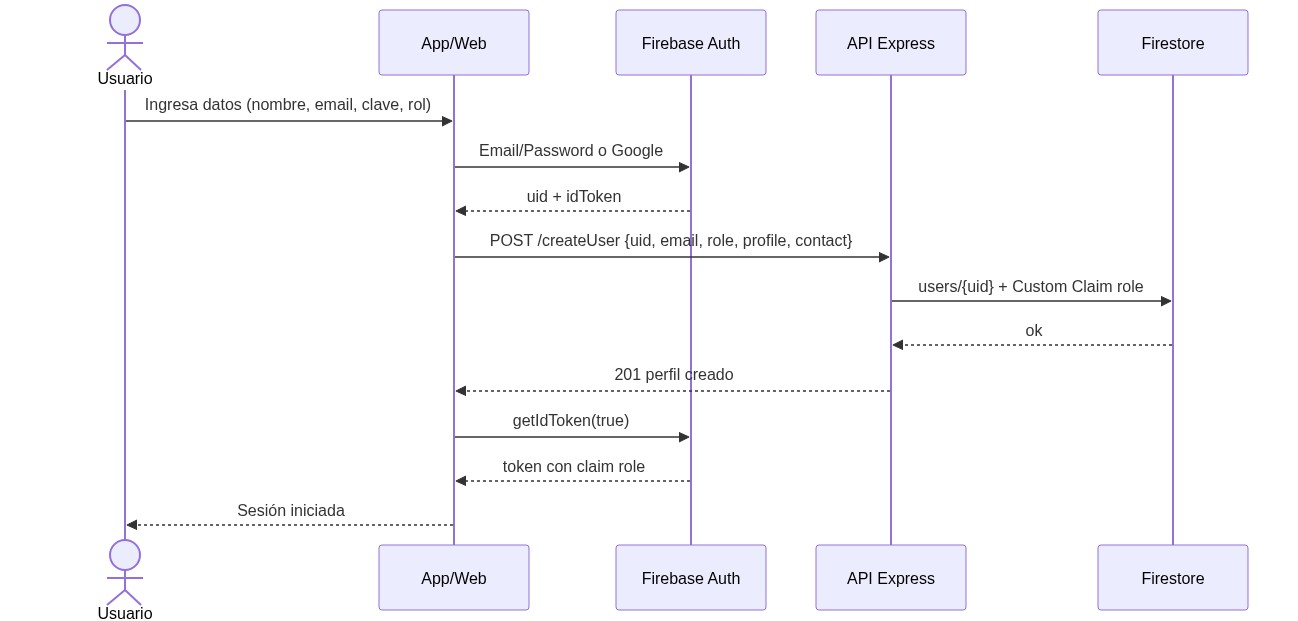
\includegraphics[width=0.72\textwidth]{figuras/registro-y-autenticacion.png}
    \captionof{figure}{Diagrama de flujo del proceso de registro y autenticación de un usuario.}
    \label{fig:registro}
\end{figure}

\subsection{Configuración del catálogo de servicios}

\begin{figure}[H]
    \centering
    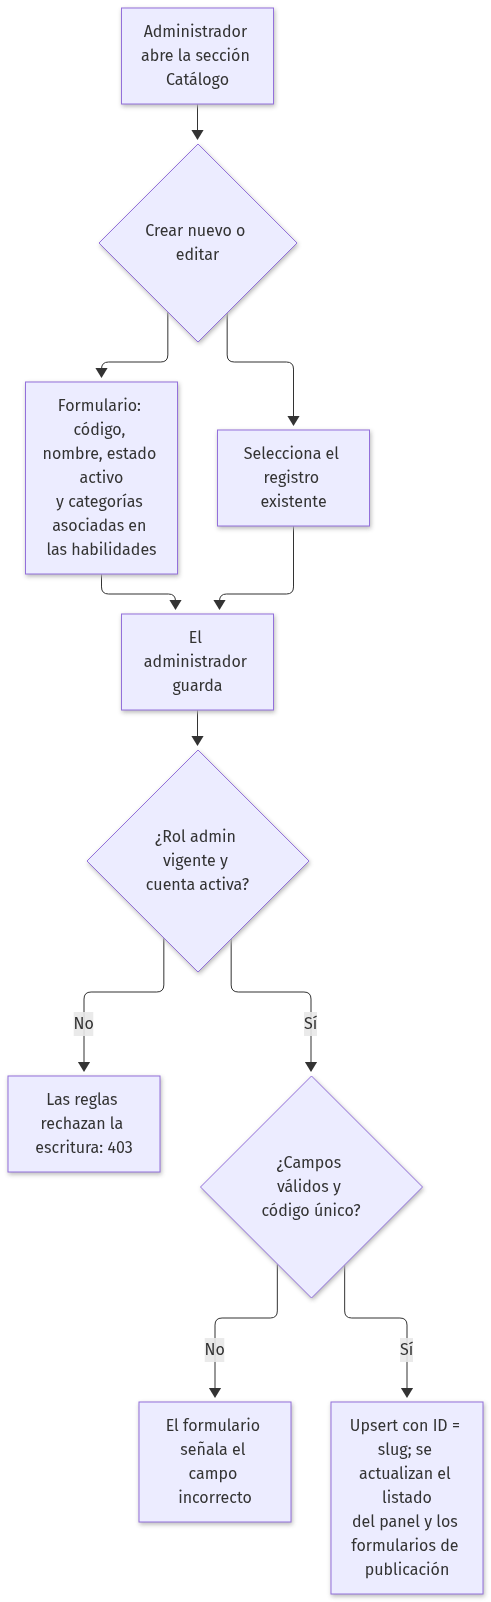
\includegraphics[width=0.72\textwidth, height=0.78\textheight, keepaspectratio]{figuras/flujo-catalogo.png}
    \captionof{figure}{Diagrama de flujo del proceso de mantenimiento del catálogo de categorías y habilidades. La lectura es pública y la escritura corresponde al administrador.}
    \label{fig:catalogo}
\end{figure}

\subsection{Publicación de un trabajo}

\begin{figure}[H]
    \centering
    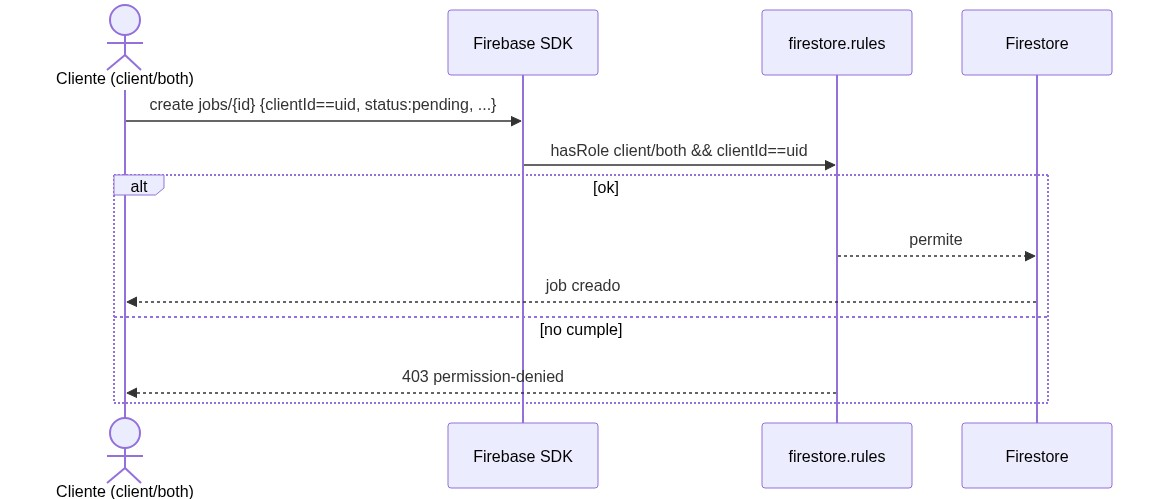
\includegraphics[width=0.72\textwidth]{figuras/publicacion-de-un-trabajo.png}
    \captionof{figure}{Diagrama de flujo del proceso de publicación de un trabajo por parte del cliente.}
    \label{fig:publicacion}
\end{figure}

\subsection{Notificación a los prestadores de servicios}

\begin{figure}[H]
    \centering
    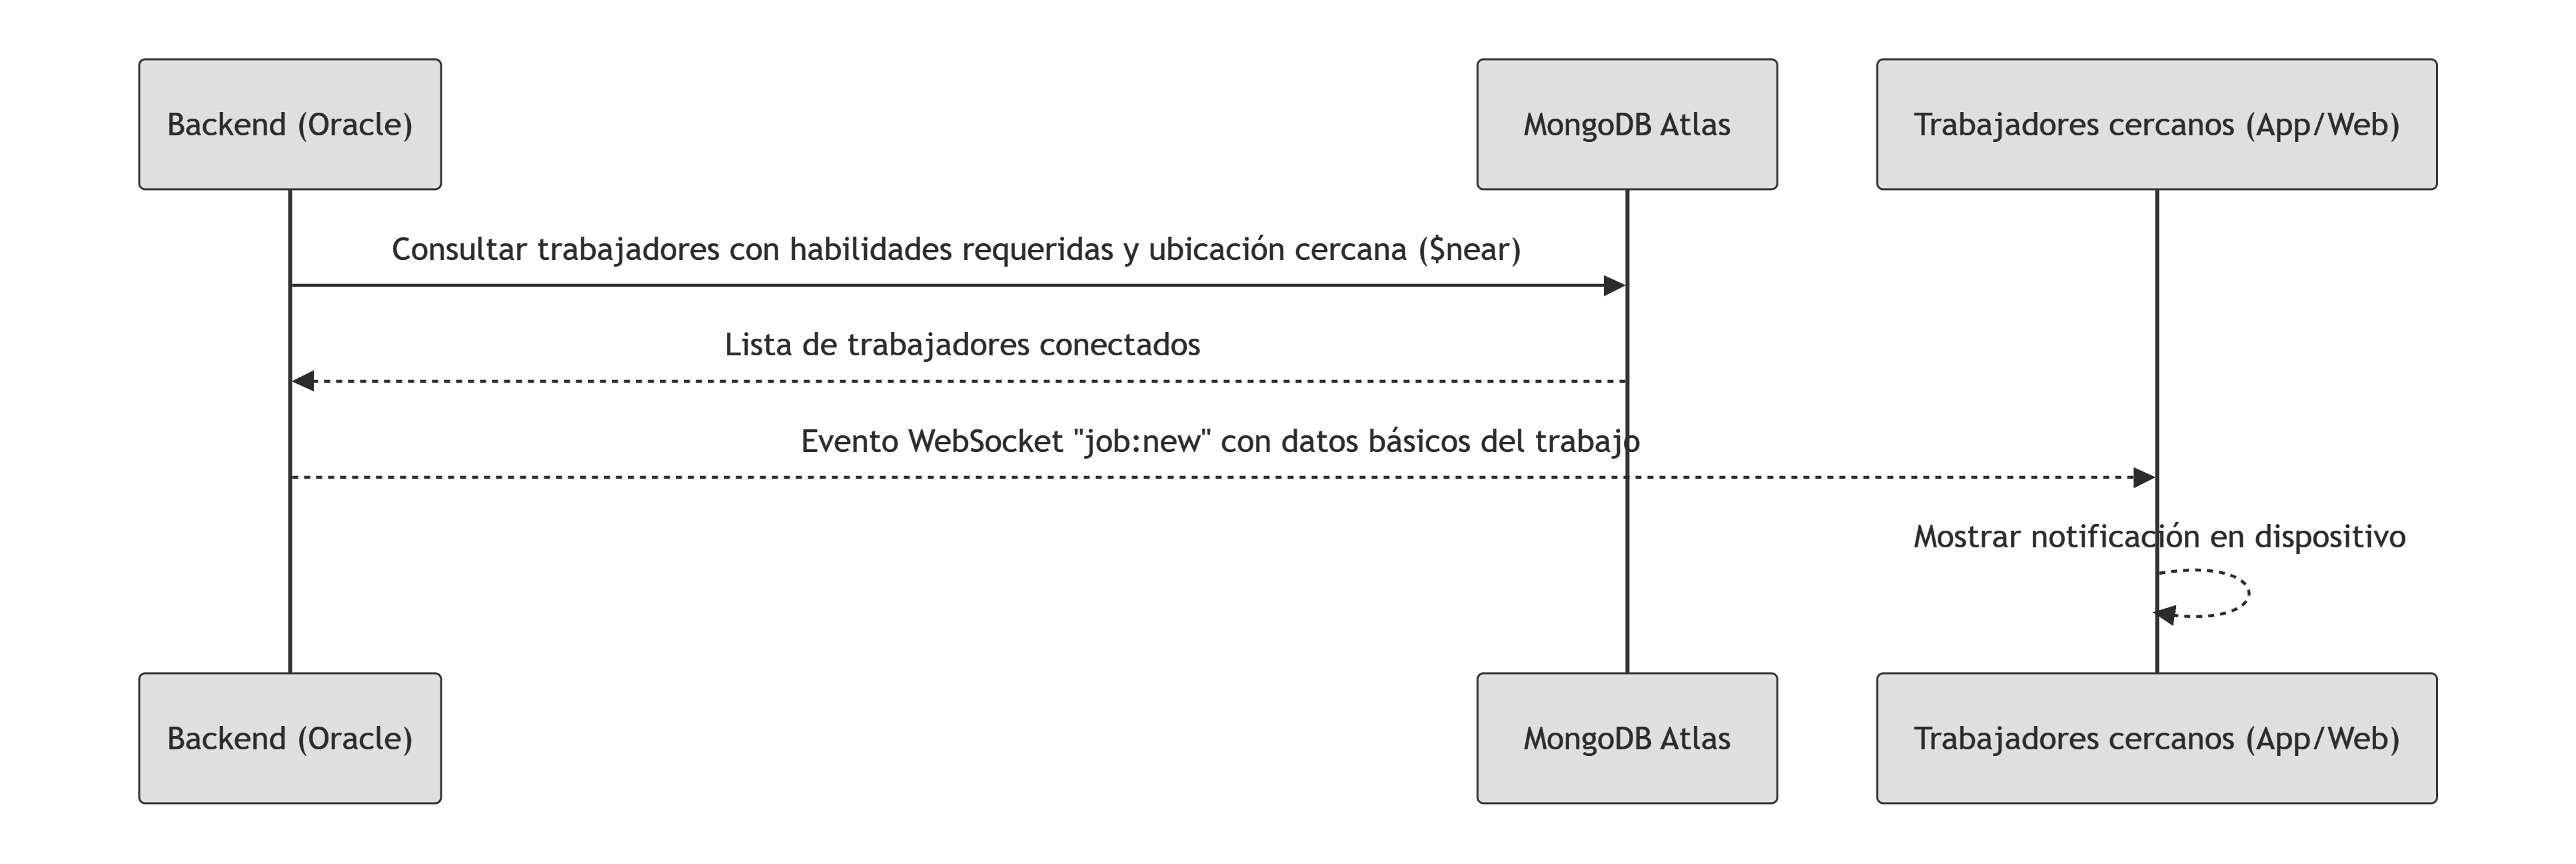
\includegraphics[width=0.72\textwidth]{figuras/notificacion-prestadores-de-servicios.png}
    \captionof{figure}{Diagrama de flujo del proceso de notificación a los trabajadores cercanos al trabajo publicado.}
    \label{fig:notificacion}
\end{figure}

\subsection{Envío de ofertas}

\begin{figure}[H]
    \centering
    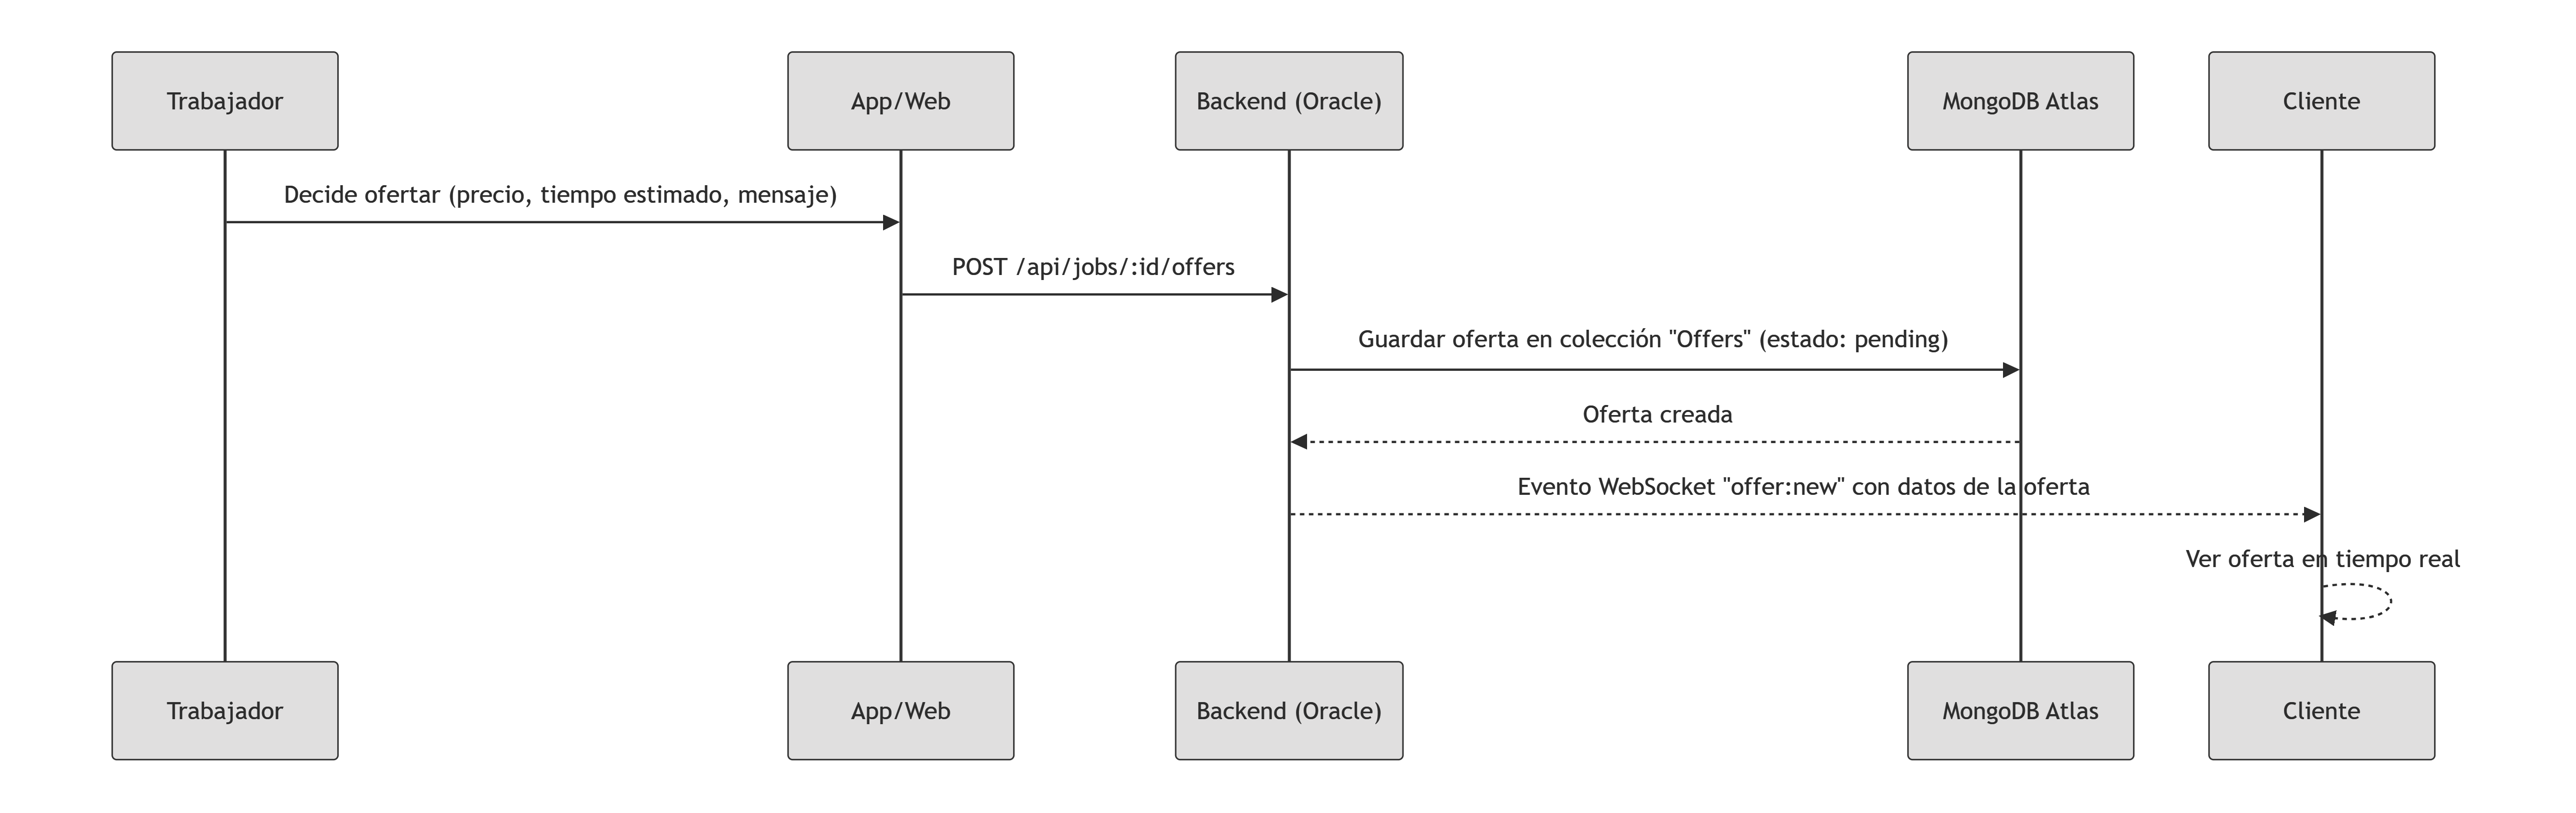
\includegraphics[width=0.72\textwidth]{figuras/envio-de-ofertas.png}
    \captionof{figure}{Diagrama de flujo del proceso de envío de una oferta por parte del trabajador.}
    \label{fig:ofertas}
\end{figure}

\subsection{Aceptación de una oferta}

\begin{figure}[H]
    \centering
    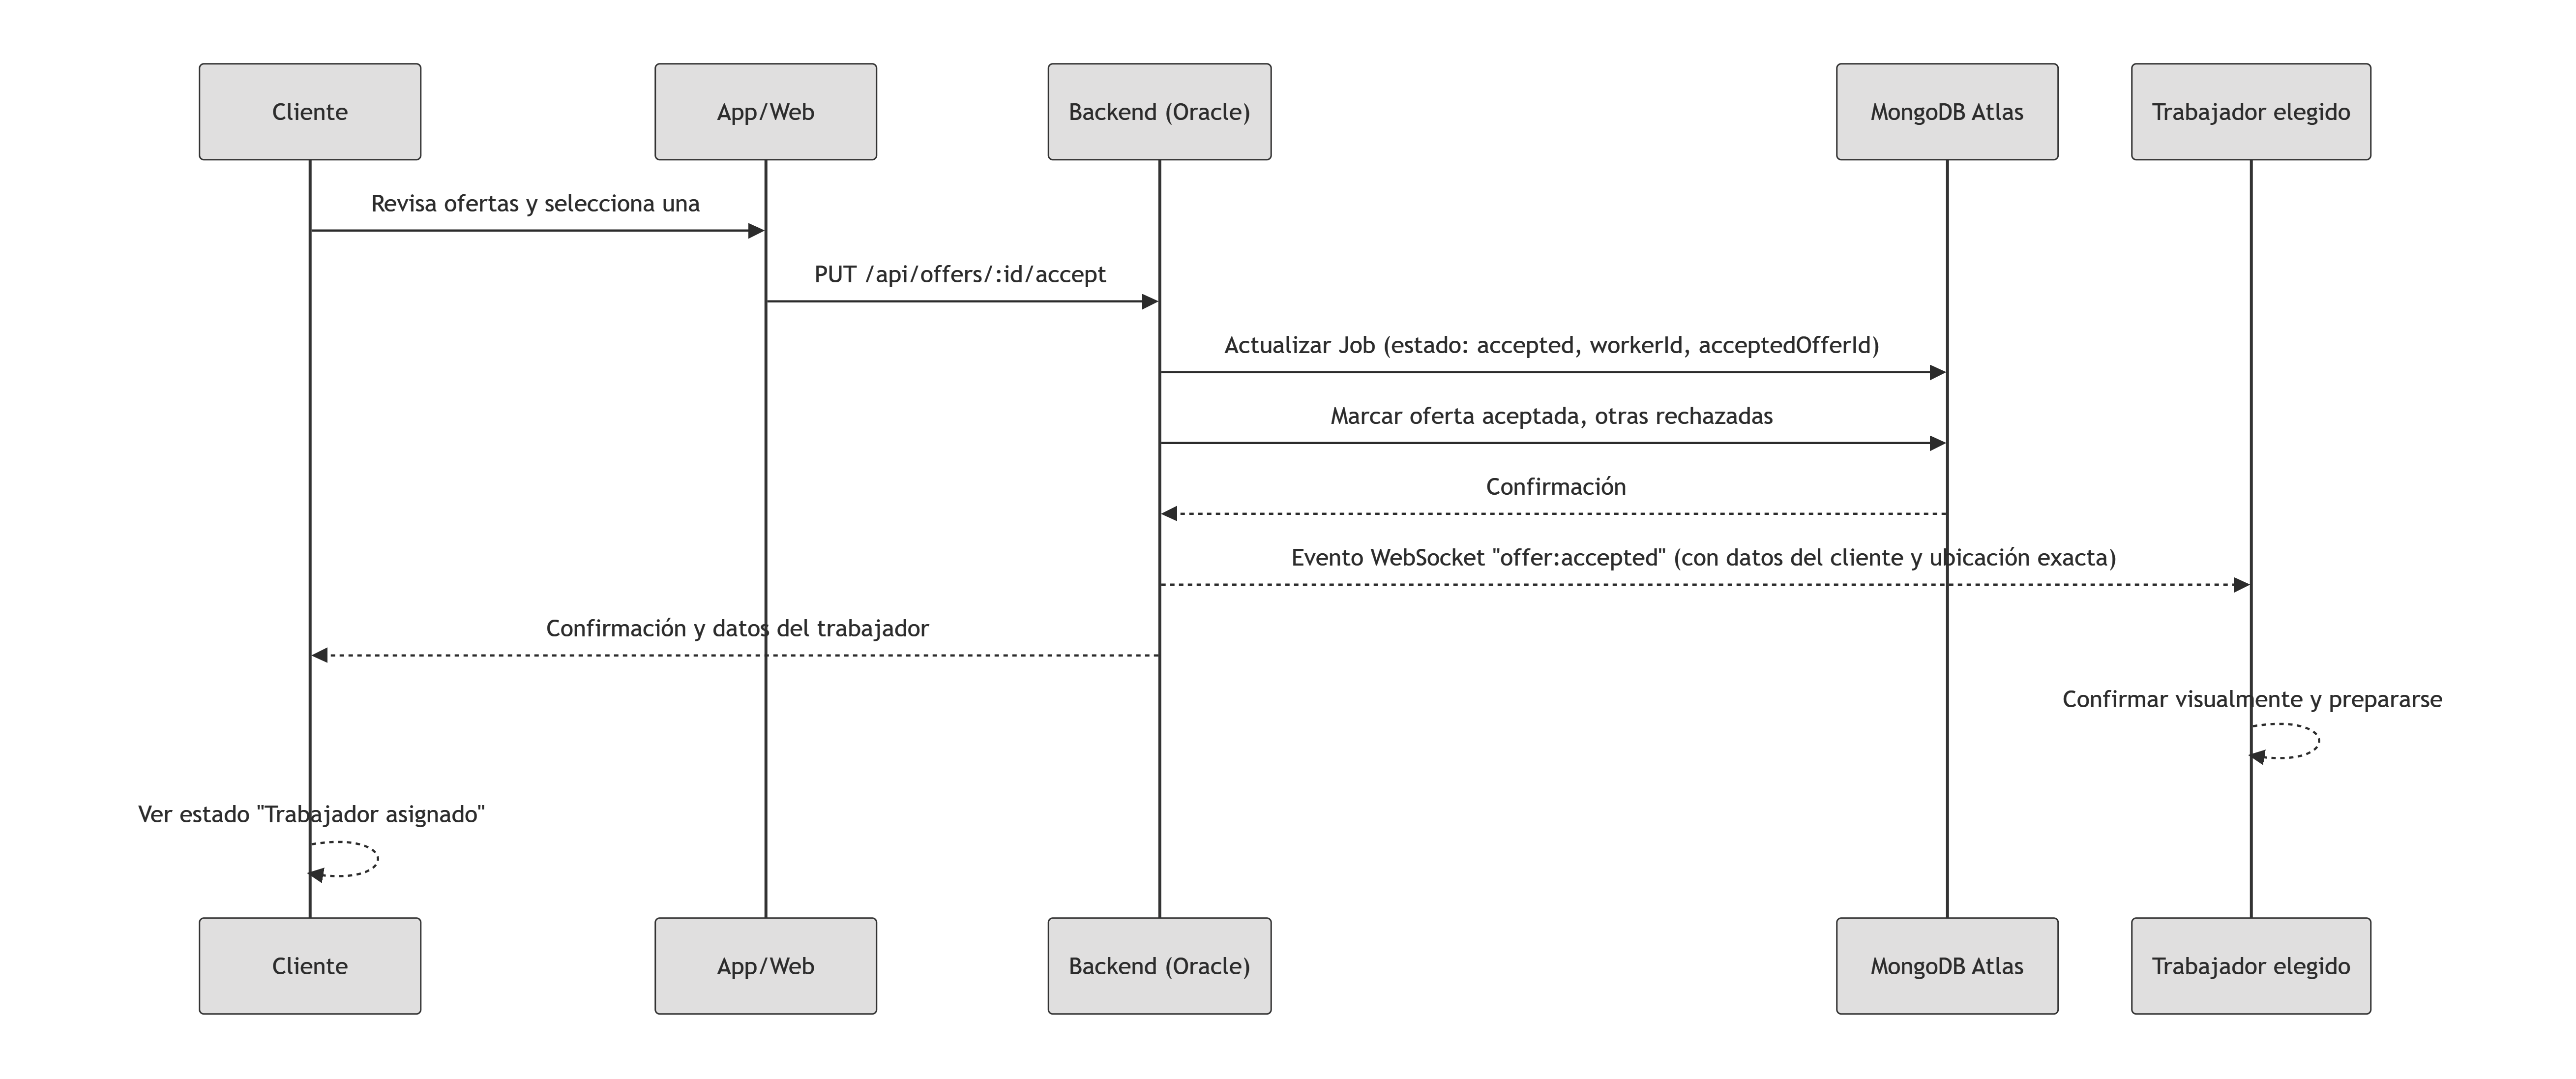
\includegraphics[width=0.72\textwidth]{figuras/aceptacion-de-una-oferta.png}
    \captionof{figure}{Diagrama de flujo del proceso de aceptación de oferta y asignación del trabajador.}
    \label{fig:aceptacion}
\end{figure}

\subsection{Ejecución de un trabajo}

\begin{figure}[H]
    \centering
    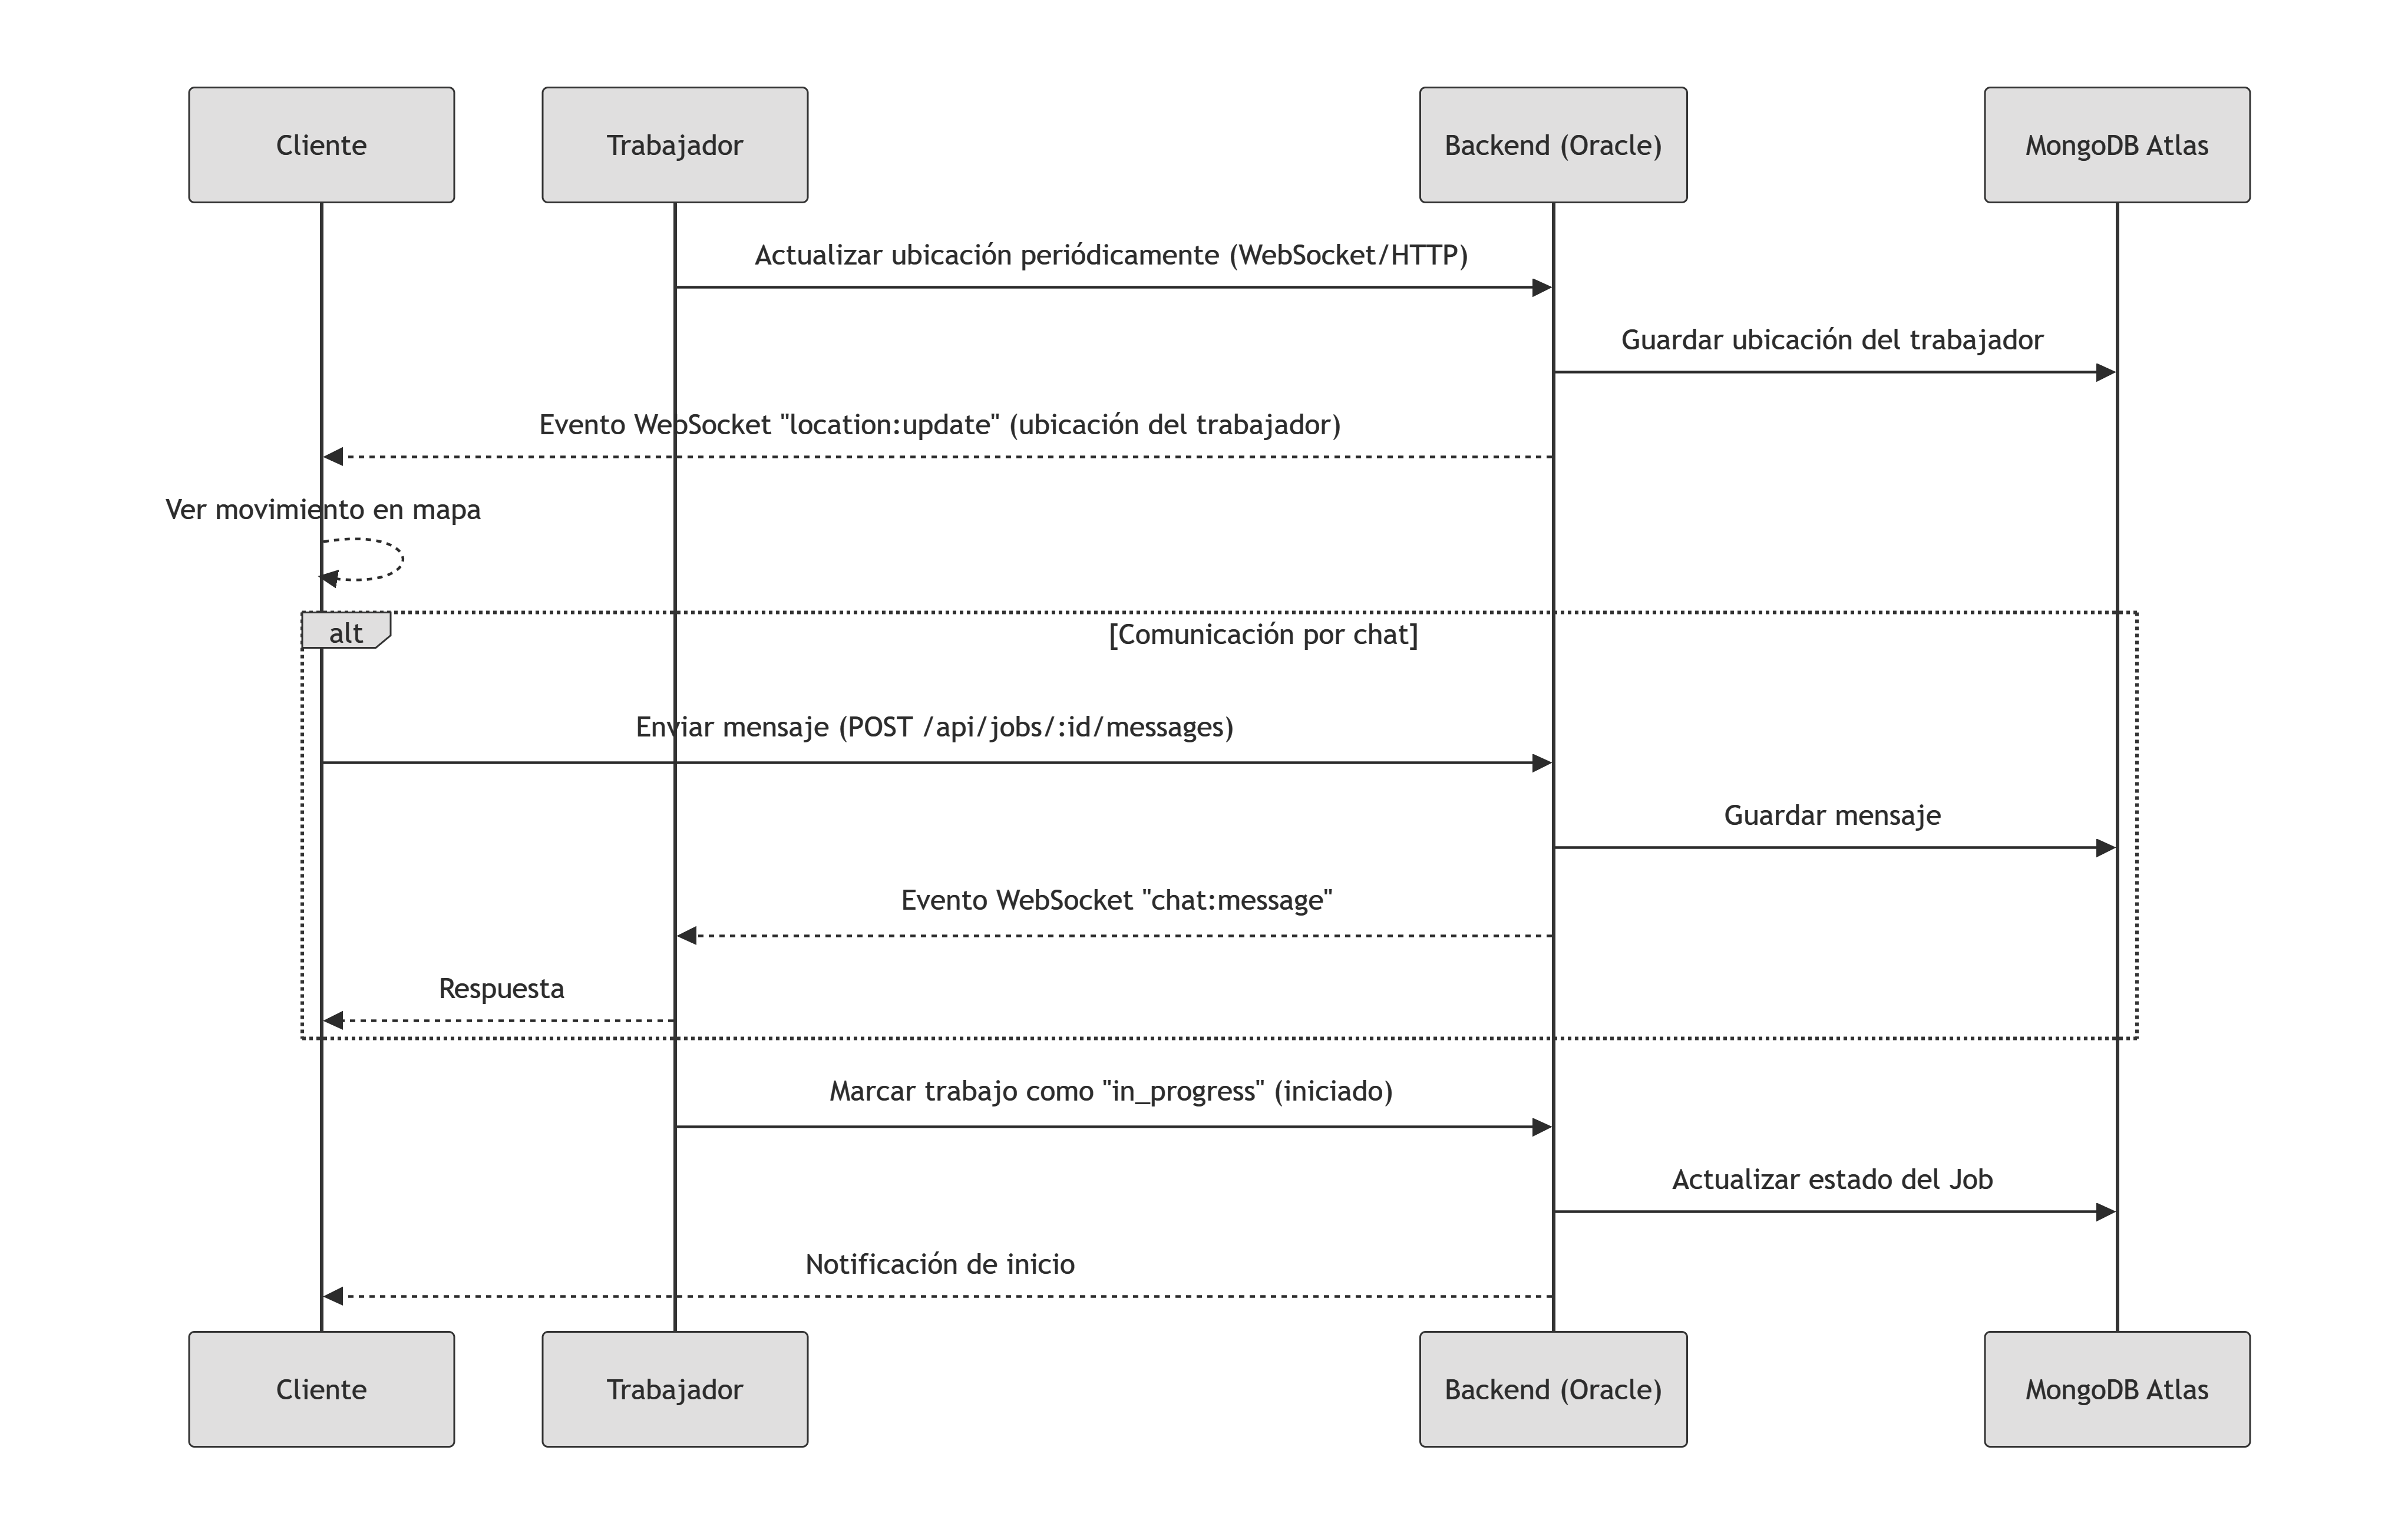
\includegraphics[width=0.72\textwidth]{figuras/ejecucion-de-un-trabajo.png}
    \captionof{figure}{Diagrama de flujo del proceso de ejecución del trabajo, seguimiento y coordinación.}
    \label{fig:ejecucion}
\end{figure}

\subsection{Conversación y coordinación}

\begin{figure}[H]
    \centering
    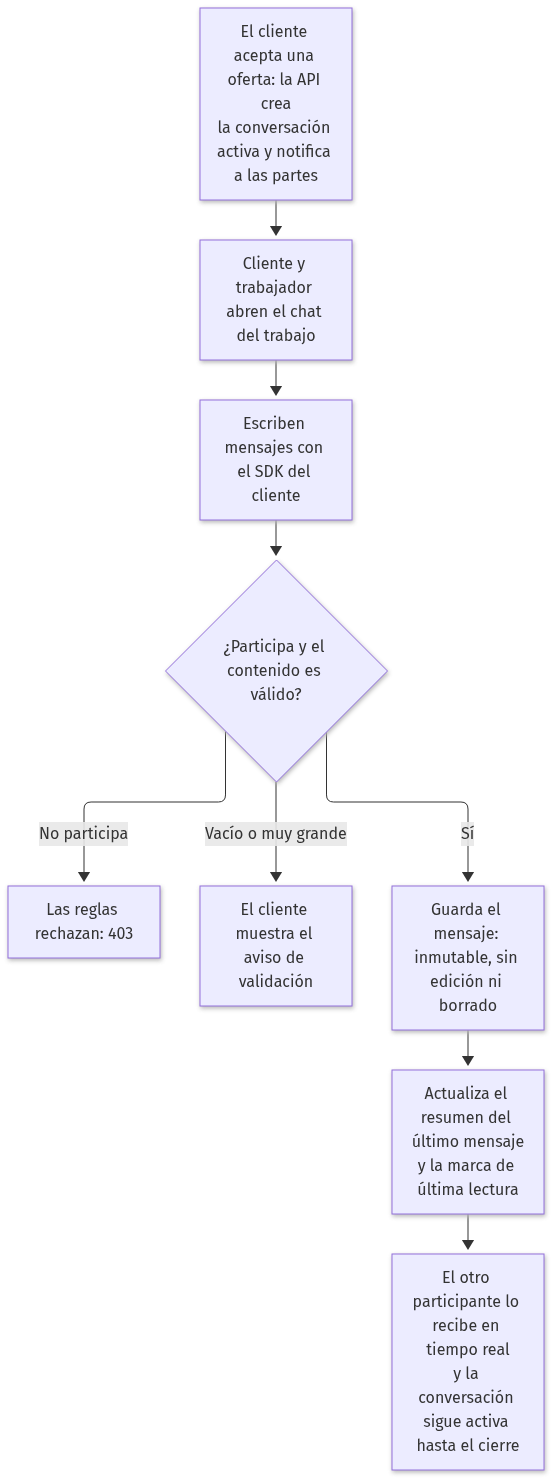
\includegraphics[width=0.72\textwidth, height=0.78\textheight, keepaspectratio]{figuras/flujo-conversacion.png}
    \captionof{figure}{Diagrama de flujo del proceso de mensajería entre cliente y trabajador dentro de la conversación del trabajo.}
    \label{fig:conversacion}
\end{figure}

\subsection{Llamada de voz entre las partes}

\begin{figure}[H]
    \centering
    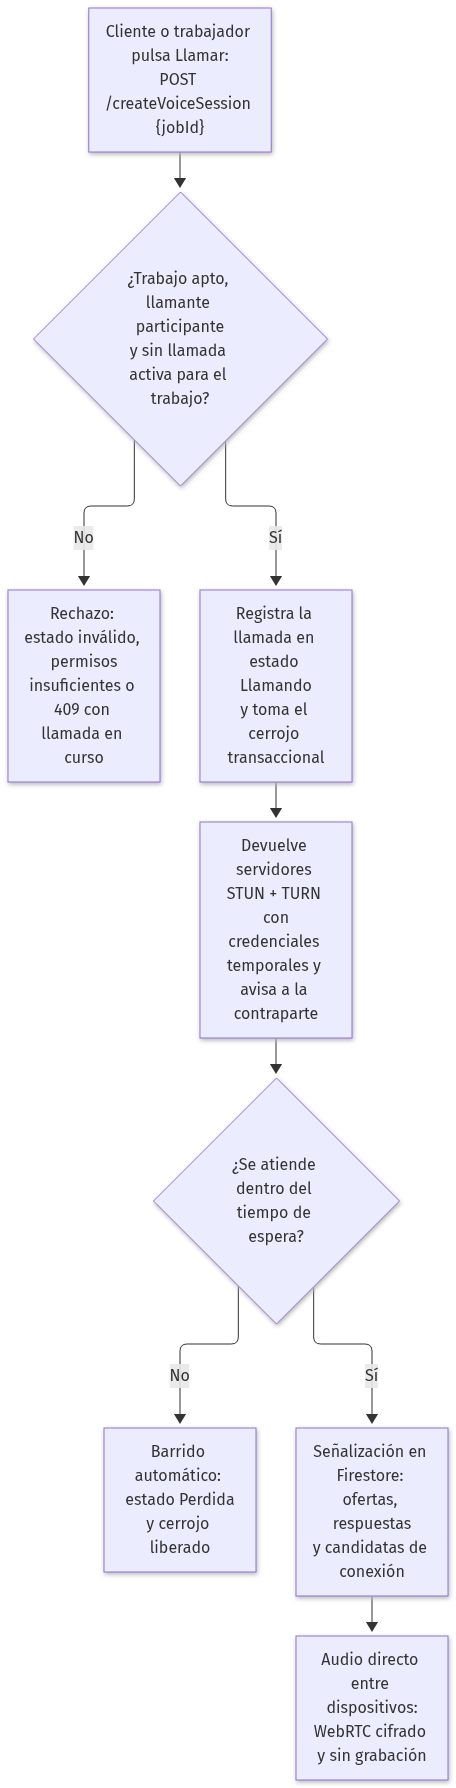
\includegraphics[width=0.72\textwidth, height=0.78\textheight, keepaspectratio]{figuras/flujo-llamada-voz-1.png}
    \captionof{figure}{Diagrama de flujo de la solicitud y el establecimiento de una llamada de voz.}
    \label{fig:llamada1}
\end{figure}

\begin{figure}[H]
    \centering
    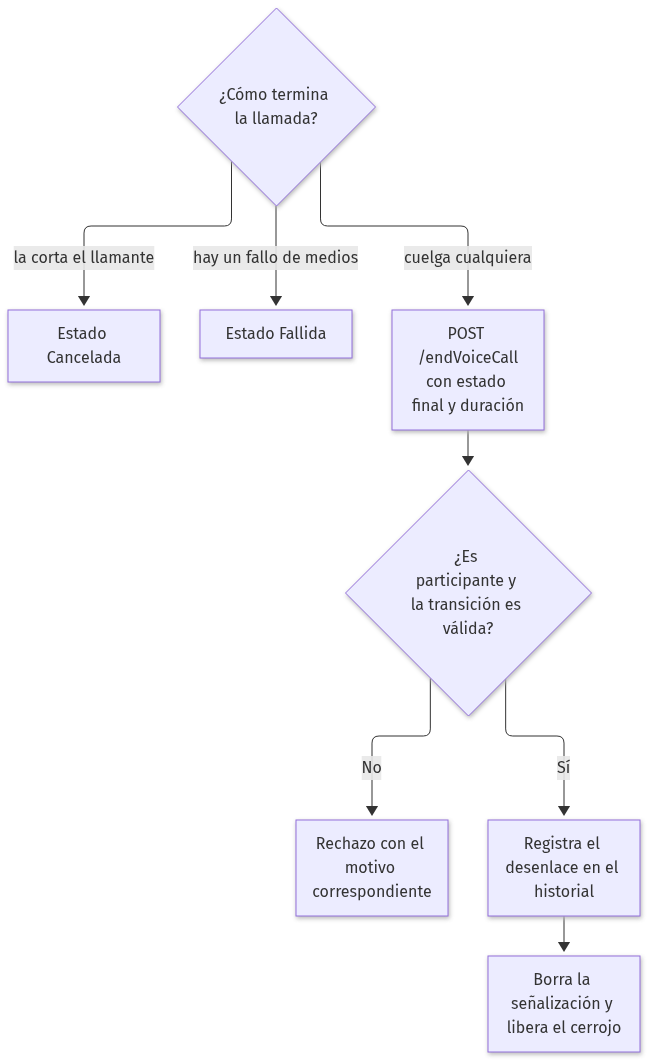
\includegraphics[width=0.72\textwidth, height=0.78\textheight, keepaspectratio]{figuras/flujo-llamada-voz-2.png}
    \captionof{figure}{Diagrama de flujo del cierre de la llamada de voz y la actualización del historial.}
    \label{fig:llamada2}
\end{figure}

\subsection{Finalización y calificación}

\begin{figure}[H]
    \centering
    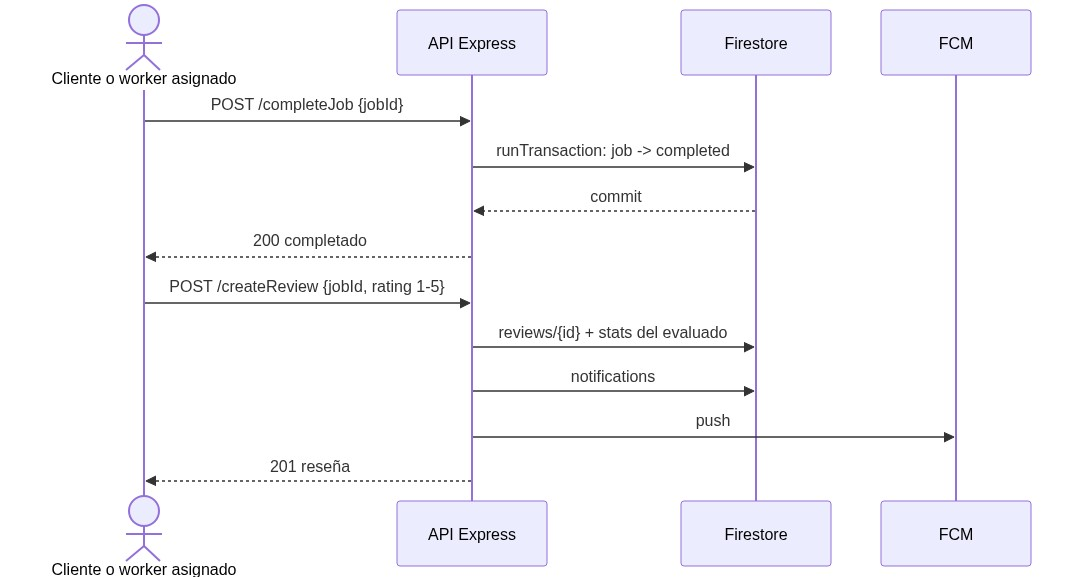
\includegraphics[width=0.72\textwidth]{figuras/finalizacion-y-calificacion.png}
    \captionof{figure}{Diagrama de flujo del proceso de finalización del trabajo y calificación de las partes.}
    \label{fig:finalizacion}
\end{figure}

\subsection{Pago simulado del trabajo}

\begin{figure}[H]
    \centering
    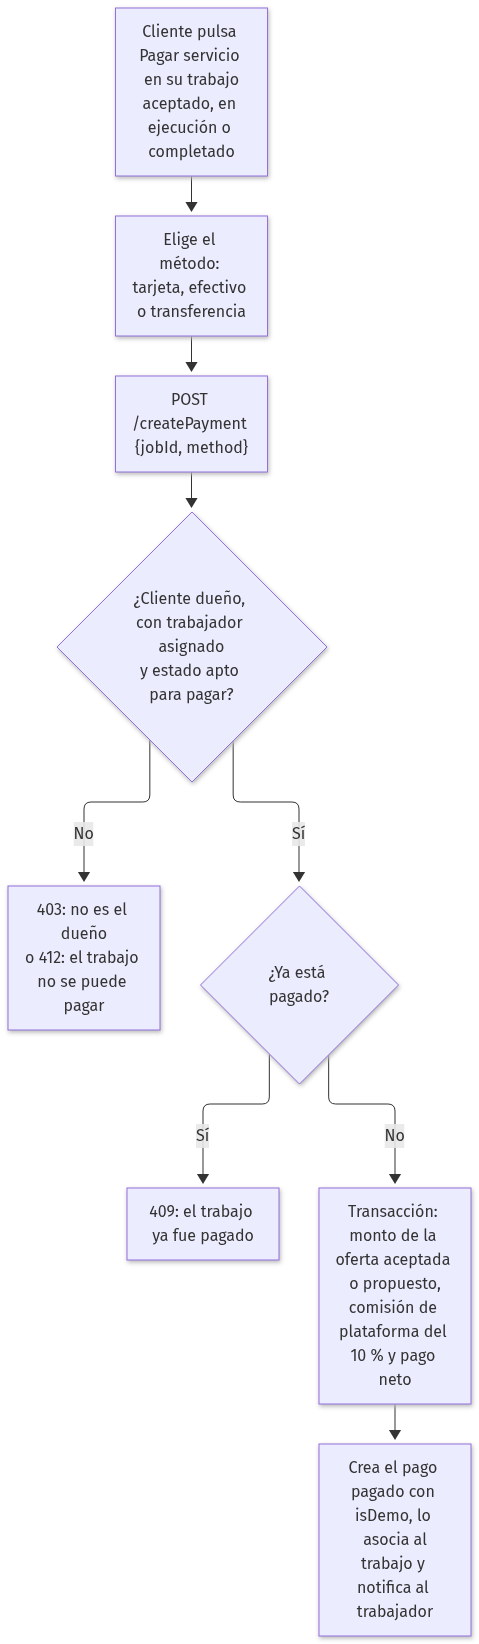
\includegraphics[width=0.72\textwidth, height=0.78\textheight, keepaspectratio]{figuras/flujo-pago.png}
    \captionof{figure}{Diagrama de flujo del registro del pago simulado del trabajo y de las validaciones que lo acompañan.}
    \label{fig:pago}
\end{figure}

\subsection{Notificaciones}

\begin{figure}[H]
    \centering
    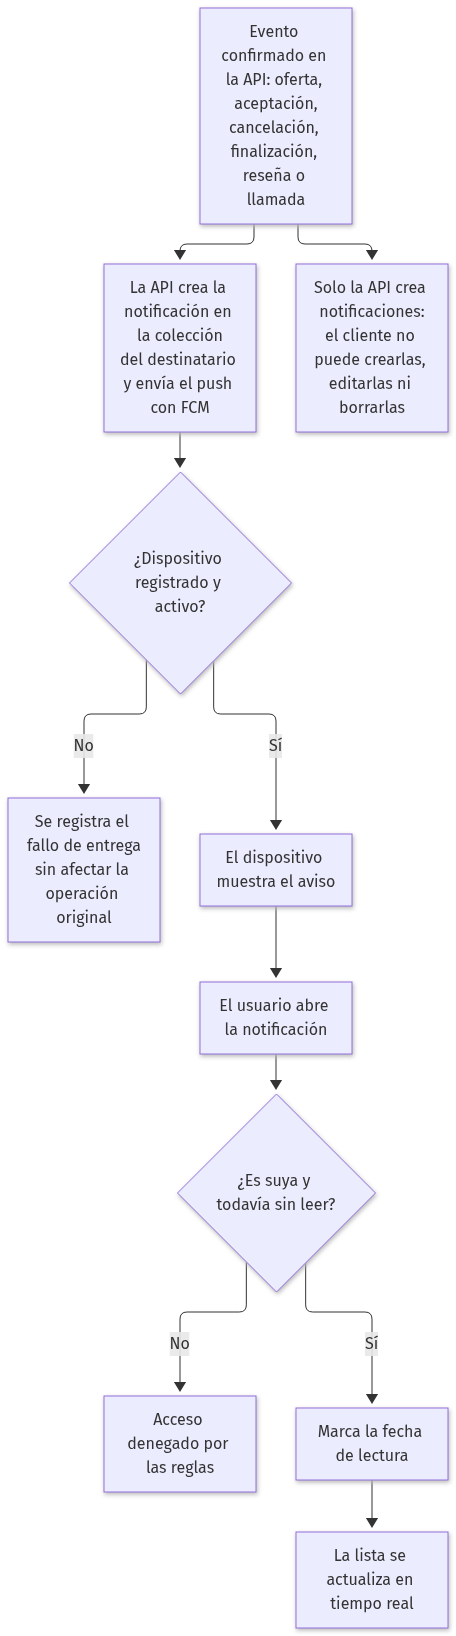
\includegraphics[width=0.72\textwidth, height=0.78\textheight, keepaspectratio]{figuras/flujo-notificaciones.png}
    \captionof{figure}{Diagrama de flujo de la creación, la entrega y la lectura de una notificación.}
    \label{fig:notificaciones}
\end{figure}

\subsection{Administración del sistema}

\begin{figure}[H]
    \centering
    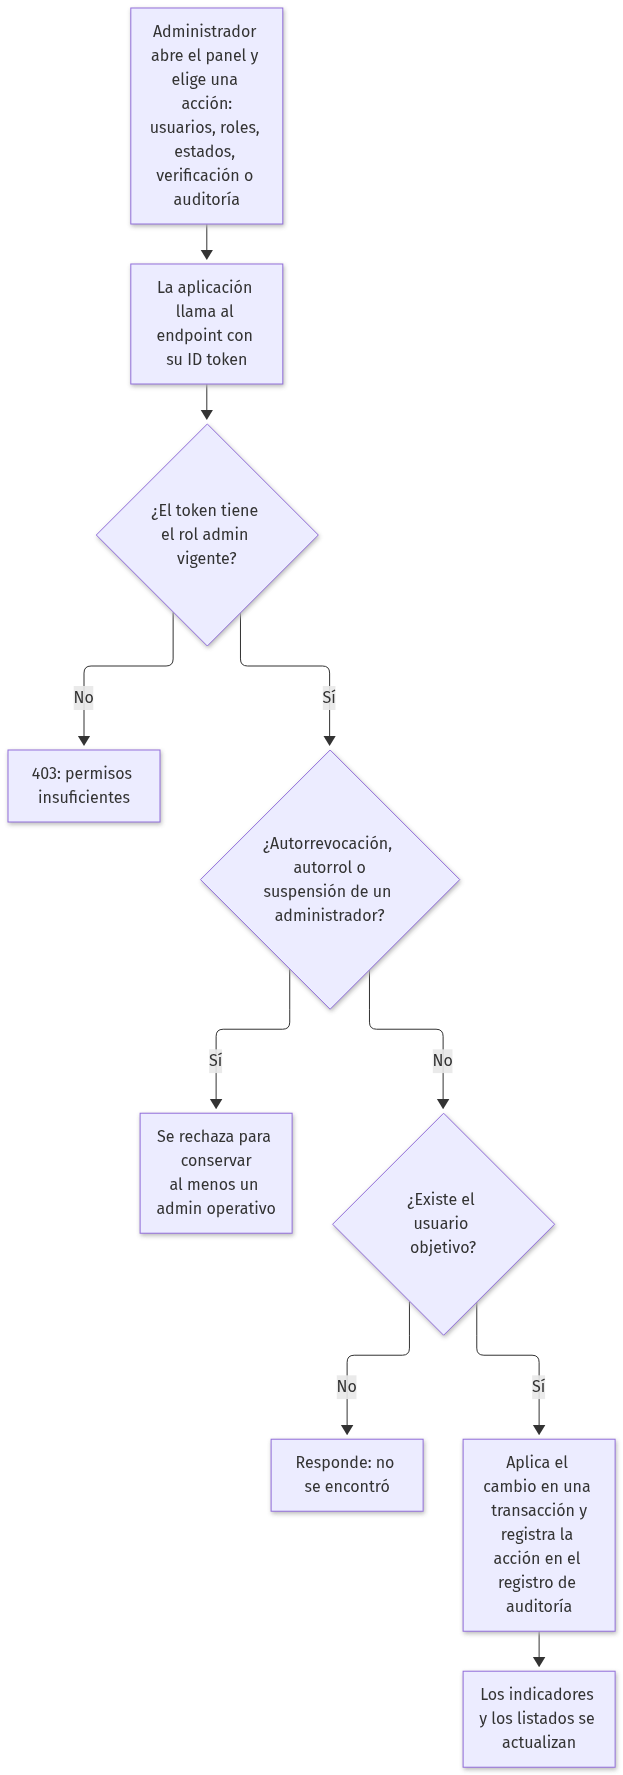
\includegraphics[width=0.72\textwidth, height=0.78\textheight, keepaspectratio]{figuras/flujo-administracion.png}
    \captionof{figure}{Diagrama de flujo de una operación administrativa y de las verificaciones de autorización que la preceden.}
    \label{fig:administracion}
\end{figure}

\subsection{Flujo general del sistema}

\begin{figure}[H]
    \centering
    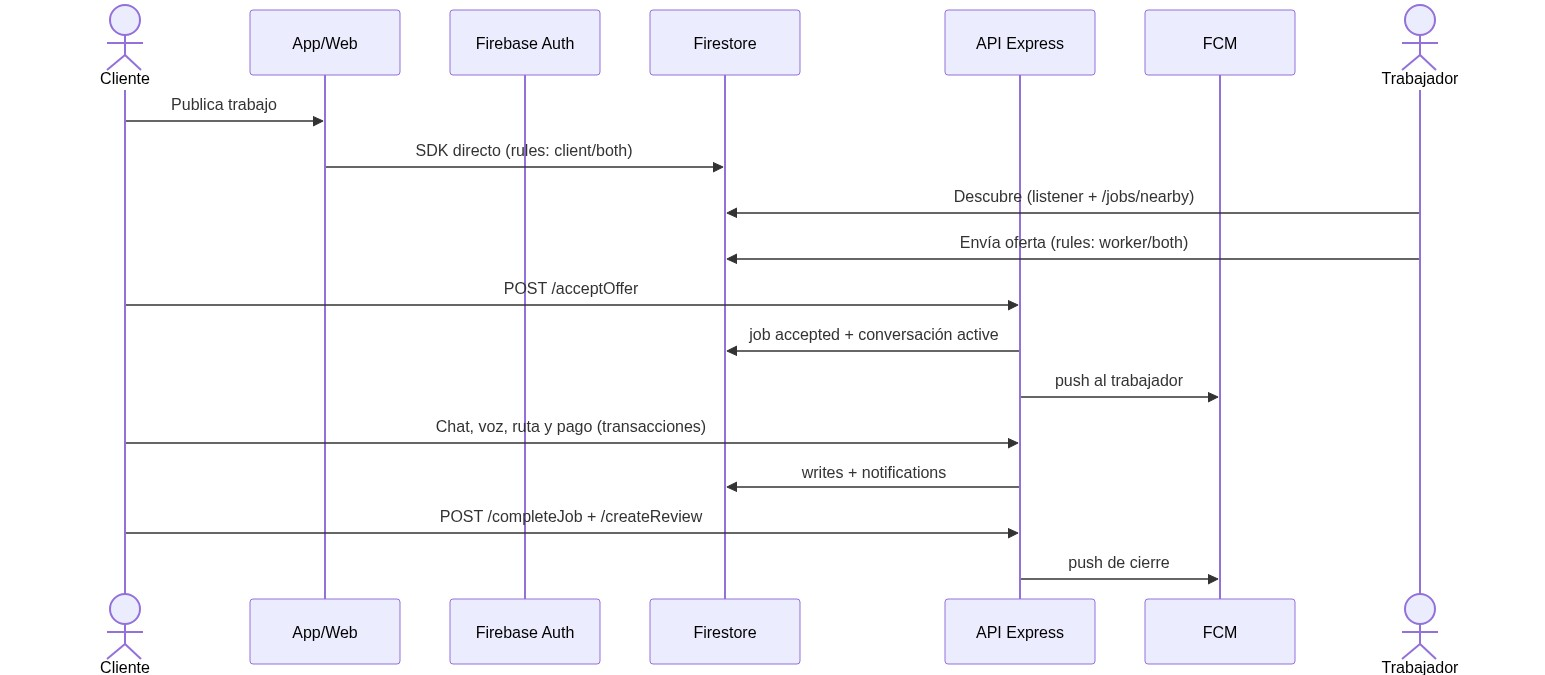
\includegraphics[width=0.8\textwidth]{figuras/flujo-general-de-sistema.png}
    \captionof{figure}{Diagrama de flujo general de la interacción entre cliente, trabajador, plataforma y servicios de soporte.}
    \label{fig:flujogeneral}
\end{figure}

\subsection{Ciclo de vida del trabajo}

\begin{figure}[H]
    \centering
    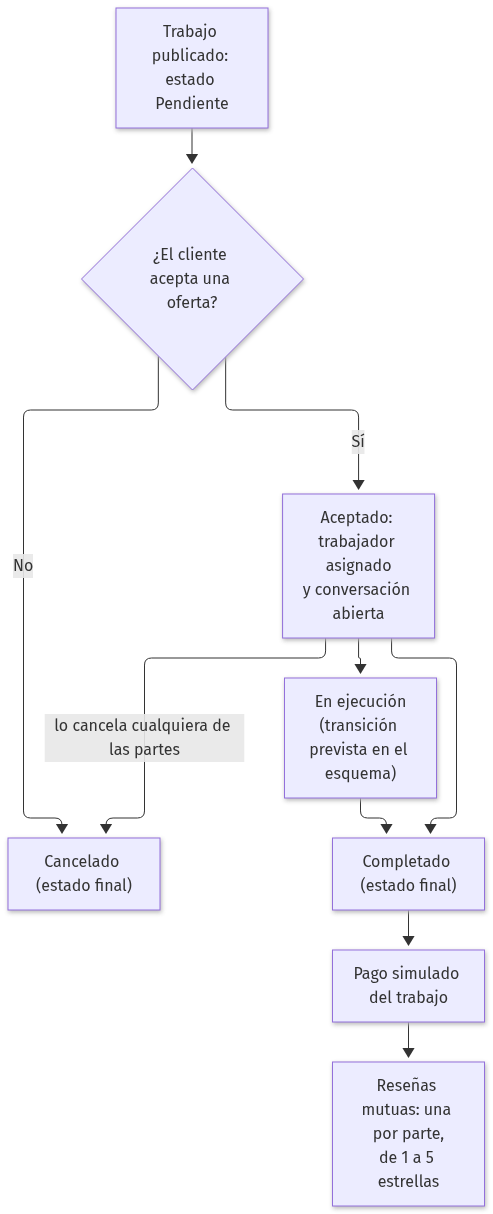
\includegraphics[width=0.62\textwidth]{figuras/ciclo-de-vida-del-trabajo.png}
    \captionof{figure}{Diagrama del ciclo de vida de un trabajo: pendiente, aceptado, completado o cancelado.}
    \label{fig:ciclo}
\end{figure}

% =====================================================================
% 6. CASOS DE USO
% =====================================================================
\section{Casos de uso}

\subsection{Diagrama de casos de uso del sistema}

\begin{figure}[H]
\centering
\resizebox{\textwidth}{!}{%
\begin{tikzpicture}[node distance=2.5cm,font=\small]
    % Actores (alineados a la izquierda)
    \node[actor] (cliente) at (0, 7.5) {Cliente};
    \node[actor] (trabajador) at (0, 3.5) {Trabajador};
    \node[actor] (ambos) at (0, -1.0) {Ambos};
    \node[actor] (admin) at (0, -8.0) {Administrador};

    % UCs de Cliente y Trabajador (Centro, x=6.5)
    \node[usecase] (cu4) at (6.5, 8.5) {UC-04 Publicar trabajo};
    \node[usecase] (cu6) at (6.5, 7.0) {UC-06 Cancelar trabajo};
    \node[usecase] (cu7) at (6.5, 5.5) {UC-07 Completar trabajo};
    \node[usecase] (cu9) at (6.5, 4.0) {UC-09 Aceptar oferta};
    \node[usecase] (cu12) at (6.5, 2.5) {UC-12 Crear reseña};
    \node[usecase] (cu15) at (6.5, 1.0) {UC-15 Iniciar llamada};
    \node[usecase] (cu16) at (6.5, -0.5) {UC-16 Finalizar llamada};
    \node[usecase] (cu10) at (6.5, -2.0) {UC-10 Calcular ruta prev.};
    \node[usecase] (cu11) at (6.5, -3.5) {UC-11 Calcular ruta of.};

    % UCs de Ambos y Admin (Derecha, x=13.0)
    \node[usecase] (cu1) at (13.0, 7.5) {UC-01 Registro/Login};
    \node[usecase] (cu2) at (13.0, 6.0) {UC-02 Crear perfil};
    \node[usecase] (cu3) at (13.0, 4.5) {UC-03 Refrescar token};
    \node[usecase] (cu5) at (13.0, 3.0) {UC-05 Buscar cercanos};
    \node[usecase] (cu8) at (13.0, 1.5) {UC-08 Enviar oferta};
    \node[usecase] (cu13) at (13.0, 0.0) {UC-13 Seguimiento y chat};
    \node[usecase] (cu14) at (13.0, -1.5) {UC-14 Notificaciones};
    
    \node[usecase] (cu17) at (13.0, -4.0) {UC-17 Panel métricas};
    \node[usecase] (cu18) at (13.0, -5.5) {UC-18 Gestionar usuarios};
    \node[usecase] (cu19) at (13.0, -7.0) {UC-19 Cambiar rol};
    \node[usecase] (cu20) at (13.0, -8.5) {UC-20 Promover admin};
    \node[usecase] (cu21) at (13.0, -10.0) {UC-21 Suspender/activar};
    \node[usecase] (cu22) at (13.0, -11.5) {UC-22 Verificar prof.};
    \node[usecase] (cu23) at (13.0, -13.0) {UC-23 Mantener catálogo};
    \node[usecase] (cu24) at (13.0, -14.5) {UC-24 Auditoría};

    % Límite del sistema
    \node[draw,fit=(cu4)(cu24),inner sep=18pt,label=above:{\textbf{PaTodo}}] (sis) {};

    % Relaciones (Usando out/in para no cruzar tanto)
    \foreach \a in {cu4,cu6,cu7,cu9,cu12,cu15,cu16} \draw[flowarrow] (cliente.east) to[out=0,in=180] (\a.west);
    \foreach \a in {cu5,cu8,cu10,cu15,cu16} \draw[flowarrow] (trabajador.east) to[out=0,in=180] (\a.west);
    \foreach \a in {cu1,cu2,cu3,cu4,cu5,cu8,cu13,cu14} \draw[flowarrow] (ambos.east) to[out=0,in=180] (\a.west);
    \foreach \a in {cu17,cu18,cu19,cu20,cu21,cu22,cu23,cu24} \draw[flowarrow] (admin.east) to[out=0,in=180] (\a.west);
\end{tikzpicture}}%
\captionof{figure}{Diagrama de casos de uso del sistema.}
\label{fig:casosdeuso}
\end{figure}

\subsection{Casos de uso del módulo de autenticación}

\subsubsection{Caso de uso ``UC-01: Registrarse / Iniciar sesión''}

\begin{longtable}{|P{3.3cm}|L{11.2cm}|}
\hline
\textbf{Descripción} & El usuario crea una cuenta nueva o inicia sesión con su correo electrónico y contraseña, o bien mediante su cuenta de Google. \\ \hline
\textbf{Actores primarios} & Cliente, Trabajador. \\ \hline
\textbf{Contexto} & Pantalla de acceso del sistema. \\ \hline
\textbf{Condiciones previas} & El usuario no tiene una sesión iniciada. \\ \hline
\textbf{Flujo básico} &
\begin{enumerate}
    \item El usuario ingresa a la aplicación y selecciona la opción de registro o de inicio de sesión.
    \item El usuario elige el método de autenticación: correo electrónico y contraseña, o Google.
    \item Si elige Google, el sistema abre la ventana de consentimiento y recibe el resultado de la autenticación del proveedor.
    \item Si elige correo y contraseña, el usuario ingresa su correo y su contraseña.
    \item El sistema verifica las credenciales contra el servicio de autenticación.
    \item Si las credenciales son válidas, el sistema genera un token de sesión y lo entrega a la aplicación.
    \item Si el método es Google y la cuenta es nueva, el sistema solicita completar el perfil (teléfono y rol).
    \item El sistema muestra la pantalla de bienvenida correspondiente al rol seleccionado.
\end{enumerate} \\ \hline
\textbf{Requerimientos especiales} & Las contraseñas nunca se almacenan en el cliente ni se envían a la API. La sesión se mantiene mediante el token de identidad. \\ \hline
\textbf{Salida} & El usuario cuenta con sesión iniciada y token de identidad válido. \\ \hline
\textbf{Excepciones} & Credenciales inválidas: se muestra un mensaje de autenticación fallida sin revelar si el correo existe. Fallo del proveedor de Google: se muestra un mensaje de error y se ofrece reintentar. \\ \hline
\end{longtable}

\subsubsection{Caso de uso ``UC-02: Crear perfil de usuario''}

\begin{longtable}{|P{3.3cm}|L{11.2cm}|}
\hline
\textbf{Descripción} & El usuario autenticado completa su perfil y selecciona el rol con el que desea operar. \\ \hline
\textbf{Actores primarios} & Cliente, Trabajador, Ambos. \\ \hline
\textbf{Contexto} & Módulo de perfil. \\ \hline
\textbf{Condiciones previas} & El usuario debe haber iniciado sesión. \\ \hline
\textbf{Flujo básico} &
\begin{enumerate}
    \item La aplicación solicita el nombre, el teléfono y el rol deseado.
    \item El usuario ingresa sus datos y selecciona el rol: cliente, trabajador o ambos.
    \item Opcionalmente, el trabajador registra sus habilidades y sus vehículos.
    \item La aplicación envía la solicitud de creación de perfil al servicio REST.
    \item El servicio verifica el token, comprueba que el identificador y el correo coincidan con los del token y comprueba que el perfil no exista previamente.
    \item El servicio crea el documento del usuario con su rol y asigna el rol como declaración personalizada en el token de identidad.
    \item La aplicación refresca el token de identidad y habilita las funciones del rol elegido.
\end{enumerate} \\ \hline
\textbf{Requerimientos especiales} & El identificador y el correo de la solicitud deben coincidir con los del token; de lo contrario se rechaza la operación. El teléfono es obligatorio. \\ \hline
\textbf{Salida} & El documento de usuario creado con su rol, y las acciones del rol habilitadas. \\ \hline
\textbf{Excepciones} & Perfil ya existente: el servicio responde \texttt{409} y la aplicación dirige al usuario a editar su perfil. \\ \hline
\end{longtable}

% ---------------------------------------------------------------------
\subsection{Casos de uso del módulo de trabajos}

\subsubsection{Caso de uso ``UC-04: Publicar trabajo''}

\begin{longtable}{|P{3.3cm}|L{11.2cm}|}
\hline
\textbf{Descripción} & El cliente publica una solicitud de servicio para recibir ofertas de trabajadores cercanos. \\ \hline
\textbf{Actores primarios} & Cliente. \\ \hline
\textbf{Contexto} & Módulo de trabajos. \\ \hline
\textbf{Condiciones previas} & El usuario debe tener rol cliente o ambos, su cuenta no debe estar suspendida y su perfil debe estar completo. \\ \hline
\textbf{Flujo básico} &
\begin{enumerate}
    \item El usuario accede a la opción de publicar un trabajo.
    \item El sistema carga el catálogo de categorías y habilidades, de lectura pública.
    \item El usuario describe el trabajo, selecciona la categoría y las habilidades requeridas.
    \item El usuario indica el lugar de la recogida; la aplicación obtiene las coordenadas del dispositivo o permite introducir la dirección.
    \item Opcionalmente, el usuario indica un punto de entrega y la fecha en que requiere el servicio.
    \item El usuario indica el precio que está dispuesto a pagar.
    \item La aplicación escribe el trabajo directamente en la base de datos, asignándolo al usuario y en estado pendiente.
    \item El sistema muestra la confirmación de publicación y el trabajo queda disponible para los trabajadores cercanos.
\end{enumerate} \\ \hline
\textbf{Requerimientos especiales} & El trabajo debe incluir los datos mínimos obligatorios: cliente, descripción, ubicación, precio y estado. La ubicación debe incluir el valor de geocodificación para que el trabajo aparezca en las búsquedas por proximidad. \\ \hline
\textbf{Salida} & Trabajo publicado en estado pendiente y visible en la búsqueda de trabajos cercanos. \\ \hline
\textbf{Excepciones} & El usuario no cuenta con permisos para publicar: se muestra un mensaje de permisos insuficientes. Los campos obligatorios incompletos se señalan en el formulario. \\ \hline
\end{longtable}

\subsubsection{Caso de uso ``UC-05: Buscar trabajos cercanos''}

\begin{longtable}{|P{3.3cm}|L{11.2cm}|}
\hline
\textbf{Descripción} & El trabajador consulta los trabajos pendientes próximos a su ubicación, filtrados por distancia y, opcionalmente, por categoría. \\ \hline
\textbf{Actores primarios} & Trabajador. \\ \hline
\textbf{Contexto} & Módulo de trabajos cercanos. \\ \hline
\textbf{Condiciones previas} & El usuario debe tener rol trabajador o ambos, su cuenta no debe estar suspendida y debe contar con ubicación disponible. \\ \hline
\textbf{Flujo básico} &
\begin{enumerate}
    \item El usuario abre la pantalla de trabajos cercanos.
    \item La aplicación obtiene las coordenadas del dispositivo y solicita la búsqueda con el radio configurado, por defecto 10 kilómetros.
    \item Opcionalmente, el usuario ajusta el radio de búsqueda o selecciona una categoría.
    \item El servicio calcula los límites geográficos del área solicitada y consulta los trabajos pendientes dentro de esos límites.
    \item El servicio descarta los trabajos cuya distancia real supera el radio y los ordena de menor a mayor distancia.
    \item La aplicación muestra la lista de trabajos con la distancia en línea recta, la categoría, el precio propuesto y la fecha requerida.
\end{enumerate} \\ \hline
\textbf{Requerimientos especiales} & El radio máximo admitido es de 50 kilómetros y el número máximo de resultados es de 50. La distancia mostrada no representa la ruta por carretera. \\ \hline
\textbf{Salida} & Listado de trabajos cercanos con su distancia, ordenado de menor a mayor. \\ \hline
\textbf{Excepciones} & Un cliente que intenta la búsqueda recibe un mensaje de permisos insuficientes. Coordenadas o radio con formato inválido: se rechaza la solicitud indicando los parámetros incorrectos. Sin trabajos en el área: se muestra un mensaje informativo. \\ \hline
\end{longtable}

\subsubsection{Caso de uso ``UC-06: Cancelar trabajo''}

\begin{longtable}{|P{3.3cm}|L{11.2cm}|}
\hline
\textbf{Descripción} & El cliente cancela un trabajo que ya no necesita, siempre que no haya sido completado. \\ \hline
\textbf{Actores primarios} & Cliente. \\ \hline
\textbf{Contexto} & Módulo de trabajos. \\ \hline
\textbf{Condiciones previas} & El usuario debe ser el cliente dueño del trabajo y el trabajo debe encontrarse en estado pendiente o aceptado. \\ \hline
\textbf{Flujo básico} &
\begin{enumerate}
    \item El usuario localiza el trabajo en su lista y selecciona la opción de cancelar.
    \item Opcionalmente, el usuario indica el motivo de la cancelación.
    \item El sistema solicita la confirmación.
    \item El usuario confirma y la aplicación envía la solicitud al servicio REST.
    \item El servicio verifica que el usuario sea el dueño del trabajo y que su estado permita la cancelación.
    \item El servicio registra la cancelación, libera los recursos asociados (seguimiento y conversación) y notifica a las partes involucradas.
\end{enumerate} \\ \hline
\textbf{Requerimientos especiales} & Un trabajo completado no puede cancelarse. La cancelación se ejecuta únicamente a través del servicio REST. \\ \hline
\textbf{Salida} & Trabajo en estado cancelado y notificación a la contraparte. \\ \hline
\textbf{Excepciones} & El usuario no es el dueño del trabajo o el estado no permite la cancelación: se rechaza la operación con el motivo correspondiente. \\ \hline
\end{longtable}

\subsubsection{Caso de uso ``UC-07: Completar trabajo''}

\begin{longtable}{|P{3.3cm}|L{11.2cm}|}
\hline
\textbf{Descripción} & Una vez prestado el servicio, el cliente o el trabajador asignado marcan el trabajo como completado. \\ \hline
\textbf{Actores primarios} & Cliente, Trabajador. \\ \hline
\textbf{Contexto} & Módulo de trabajos. \\ \hline
\textbf{Condiciones previas} & El trabajo debe encontrarse en estado aceptado y el usuario debe ser el cliente o el trabajador asignado. \\ \hline
\textbf{Flujo básico} &
\begin{enumerate}
    \item El usuario abre el detalle del trabajo y selecciona la opción de completar.
    \item El sistema solicita la confirmación.
    \item El usuario confirma y la aplicación envía la solicitud al servicio REST.
    \item El servicio verifica la participación del usuario y el estado del trabajo.
    \item El servicio registra la finalización con la fecha, libera el seguimiento de ubicación y genera las notificaciones para ambas partes.
    \item Ambas partes pueden proceder a calificar el servicio.
\end{enumerate} \\ \hline
\textbf{Requerimientos especiales} & La finalización solo es válida para trabajos aceptados. Un trabajo cancelado no puede completarse. \\ \hline
\textbf{Salida} & Trabajo en estado completado, con la fecha de finalización registrada. \\ \hline
\textbf{Excepciones} & Usuario no participante o estado inválido: se rechaza la operación. \\ \hline
\end{longtable}

% ---------------------------------------------------------------------
\subsection{Casos de uso del módulo de ofertas}

\subsubsection{Caso de uso ``UC-08: Enviar oferta''}

\begin{longtable}{|P{3.3cm}|L{11.2cm}|}
\hline
\textbf{Descripción} & El trabajador envía una oferta para un trabajo cercano, con un precio, un tiempo estimado y un mensaje para el cliente. \\ \hline
\textbf{Actores primarios} & Trabajador. \\ \hline
\textbf{Contexto} & Módulo de ofertas. \\ \hline
\textbf{Condiciones previas} & El usuario debe tener rol trabajador o ambos, su cuenta no debe estar suspendida y el trabajo debe estar pendiente y pertenecer a otro cliente. \\ \hline
\textbf{Flujo básico} &
\begin{enumerate}
    \item El trabajador selecciona un trabajo del listado de cercanos y revisa su detalle, distancia y precio propuesto.
    \item Opcionalmente, consulta la vista previa de la ruta para valorar el trayecto.
    \item El trabajador selecciona la opción de ofertar.
    \item El trabajador ingresa el precio que propone, el tiempo estimado de ejecución y un mensaje para el cliente.
    \item La aplicación escribe la oferta directamente en la base de datos, en estado pendiente.
    \item El cliente recibe una notificación de la nueva oferta y puede revisarla junto con las demás.
\end{enumerate} \\ \hline
\textbf{Requerimientos especiales} & La oferta debe incluir trabajo, trabajador, precio, tiempo estimado y estado. No se puede ofertar por un trabajo propio ni por un trabajo que ya no esté pendiente. No es posible modificar el trabajo ni el trabajador de la oferta. \\ \hline
\textbf{Salida} & Oferta registrada en estado pendiente y notificación al cliente. \\ \hline
\textbf{Excepciones} & El trabajo pertenece al propio trabajador, no está pendiente o el usuario no tiene permisos: se rechaza la oferta con el motivo correspondiente. \\ \hline
\end{longtable}

\subsubsection{Caso de uso ``UC-09: Aceptar oferta''}

\begin{longtable}{|P{3.3cm}|L{11.2cm}|}
\hline
\textbf{Descripción} & El cliente selecciona la mejor oferta, asigna al trabajador y abre la conversación de coordinación. \\ \hline
\textbf{Actores primarios} & Cliente. \\ \hline
\textbf{Contexto} & Detalle del trabajo, sección de ofertas recibidas. \\ \hline
\textbf{Condiciones previas} & El usuario debe ser el cliente dueño del trabajo, el trabajo debe estar pendiente y debe existir al menos una oferta. \\ \hline
\textbf{Flujo básico} &
\begin{enumerate}
    \item El cliente abre el detalle del trabajo y revisa las ofertas recibidas (precio, tiempo estimado, mensaje, perfil y calificación del trabajador).
    \item El cliente selecciona la oferta que desea aceptar.
    \item El sistema solicita la confirmación.
    \item El cliente confirma y la aplicación envía la solicitud al servicio REST.
    \item El servicio ejecuta una transacción que marca la oferta seleccionada como aceptada, el resto de ofertas como rechazadas y el trabajo como aceptado, registrando al trabajador asignado.
    \item El servicio crea la conversación privada entre ambas partes en estado activa.
    \item El servicio notifica la asignación al trabajador y notifica al cliente.
\end{enumerate} \\ \hline
\textbf{Requerimientos especiales} & La operación es atómica: si la transacción falla, ninguno de los cambios se aplica, evitando trabajos aceptados sin trabajador asignado. \\ \hline
\textbf{Salida} & Trabajo aceptado con trabajador asignado, conversación creada y notificaciones enviadas. \\ \hline
\textbf{Excepciones} & El trabajo ya fue aceptado por otro usuario: la operación se rechaza por conflicto. El usuario no es el dueño del trabajo: se rechaza por permisos insuficientes. \\ \hline
\end{longtable}

% ---------------------------------------------------------------------
\subsection{Casos de uso del módulo de rutas}

\subsubsection{Caso de uso ``UC-10: Calcular ruta (vista previa)''}

\begin{longtable}{|P{3.3cm}|L{11.2cm}|}
\hline
\textbf{Descripción} & El trabajador no asignado consulta la distancia y el trayecto desde su ubicación hasta un trabajo pendiente, para decidir si le interesa. \\ \hline
\textbf{Actores primarios} & Trabajador. \\ \hline
\textbf{Contexto} & Detalle de un trabajo pendiente. \\ \hline
\textbf{Condiciones previas} & El usuario debe tener rol trabajador o ambos, el trabajo debe estar pendiente y el trabajador debe tener una ubicación válida. \\ \hline
\textbf{Flujo básico} &
\begin{enumerate}
    \item El trabajador solicita calcular la ruta hacia el trabajo.
    \item La aplicación envía la solicitud al servicio REST.
    \item El servicio verifica el rol y el estado del trabajo, y comprueba la disponibilidad de la ubicación del trabajador.
    \item El servicio consulta al motor de cálculo de rutas la geometría, la distancia y la duración del trayecto.
    \item La aplicación muestra la ruta trazada sobre el mapa, con la distancia y el tiempo estimado.
\end{enumerate} \\ \hline
\textbf{Requerimientos especiales} & En este modo \textbf{no se persiste ningún dato} del trabajo ni del trabajador. \\ \hline
\textbf{Salida} & Vista previa de la ruta mostrada en pantalla. \\ \hline
\textbf{Excepciones} & El trabajador no tiene ubicación disponible: se rechaza la operación indicando que debe actualizar su ubicación. El trabajo ya está aceptado: se rechaza por estado inválido. El motor de rutas no responde: se informa que el servicio no está disponible temporalmente. \\ \hline
\end{longtable}

\subsubsection{Caso de uso ``UC-11: Calcular ruta oficial''}

\begin{longtable}{|P{3.3cm}|L{11.2cm}|}
\hline
\textbf{Descripción} & Con el trabajo ya aceptado, se calcula y almacena la ruta definitiva que sigue el trabajador, dividida en el trayecto hacia la recogida y, si existe, hacia el punto de entrega. \\ \hline
\textbf{Actores primarios} & Cliente, Trabajador. \\ \hline
\textbf{Contexto} & Detalle de un trabajo aceptado. \\ \hline
\textbf{Condiciones previas} & El trabajo debe estar aceptado y el usuario debe ser el cliente dueño o el trabajador asignado. \\ \hline
\textbf{Flujo básico} &
\begin{enumerate}
    \item El usuario solicita la ruta del trabajo aceptado.
    \item El servicio verifica la participación del usuario y el estado del trabajo.
    \item El servicio obtiene la ubicación actual del trabajador asignado y las coordenadas del trabajo.
    \item El servicio consulta al motor de rutas la geometría, la distancia y la duración; si existe destino, divide el trayecto en dos tramos.
    \item El servicio almacena el resultado en el campo de ruta del trabajo.
    \item La aplicación muestra la ruta y la distancia estimada de llegada.
\end{enumerate} \\ \hline
\textbf{Requerimientos especiales} & La ruta almacenada incluye geometría, distancia, duración, tramos, origen del dato y fecha de cálculo. \\ \hline
\textbf{Salida} & Ruta oficial almacenada en el trabajo y disponible para el cliente. \\ \hline
\textbf{Excepciones} & El trabajo no está aceptado o el usuario no participa: se rechaza la operación. Falta de ubicación del trabajador: se rechaza indicando que debe actualizar su ubicación. \\ \hline
\end{longtable}

\subsection{Casos de uso del módulo de finalización}

\subsubsection{Caso de uso ``UC-12: Crear reseña''}

\begin{longtable}{|P{3.3cm}|L{11.2cm}|}
\hline
\textbf{Descripción} & Tras completar el trabajo, el cliente y el trabajador califican mutuamente el servicio prestado. \\ \hline
\textbf{Actores primarios} & Cliente, Trabajador. \\ \hline
\textbf{Contexto} & Detalle de un trabajo completado. \\ \hline
\textbf{Condiciones previas} & El trabajo debe estar completado y el usuario debe haber participado en él sin haber publicado ya una reseña. \\ \hline
\textbf{Flujo básico} &
\begin{enumerate}
    \item El usuario abre el detalle de un trabajo completado y selecciona la opción de calificar.
    \item El usuario asigna una puntuación de una a cinco estrellas.
    \item Opcionalmente, el usuario escribe un comentario.
    \item La aplicación envía la calificación al servicio REST.
    \item El servicio verifica la participación, el estado del trabajo y que no exista ya una reseña del mismo autor para ese trabajo.
    \item El servicio registra la reseña, recalcula la calificación promedio y el número de reseñas del perfil del evaluado.
    \item El servicio notifica la nueva reseña a la contraparte.
\end{enumerate} \\ \hline
\textbf{Requerimientos especiales} & La puntuación va de 1 a 5. Las reseñas son inmutables: una vez registradas no pueden modificarse ni eliminarse. \\ \hline
\textbf{Salida} & Reseña registrada, calificación promedio del perfil actualizada y notificación a la contraparte. \\ \hline
\textbf{Excepciones} & El usuario no participó en el trabajo, el trabajo no está completado o ya lo ha calificado previamente: se rechaza la operación indicando el motivo. \\ \hline
\end{longtable}

% ---------------------------------------------------------------------
% ---------------------------------------------------------------------
\subsection{Casos de uso del módulo de seguimiento y chat}

\subsubsection{Caso de uso ``UC-13: Seguimiento en tiempo real y chat''}

\begin{longtable}{|P{3.3cm}|L{11.2cm}|}
\hline
\textbf{Descripción} & Durante la ejecución del trabajo, el trabajador reporta su ubicación y el cliente la sigue en tiempo real; además, ambas partes se comunican por mensajes dentro de la conversación del trabajo. \\ \hline
\textbf{Actores primarios} & Cliente, Trabajador. \\ \hline
\textbf{Contexto} & Detalle del trabajo en ejecución. \\ \hline
\textbf{Condiciones previas} & El trabajo debe estar aceptado y existir una conversación asociada. \\ \hline
\textbf{Flujo básico} &
\begin{enumerate}
    \item El trabajador inicia el trayecto y activa el reporte de ubicación.
    \item La aplicación escribe la posición actual del trabajador en el documento de seguimiento del trabajo.
    \item El cliente, con el detalle del trabajo abierto, observa la posición actualizada automáticamente.
    \item El trabajador puede enviar mensajes desde el chat del trabajo.
    \item La aplicación escribe el mensaje en la conversación y actualiza el resumen del último mensaje.
    \item El cliente recibe la actualización del chat en tiempo real y puede responder.
\end{enumerate} \\ \hline
\textbf{Requerimientos especiales} & El documento de seguimiento es único por trabajo (posición actual, sin historial) y se elimina al completar o cancelar. Solo el cliente dueño y el trabajador asignado pueden leer y escribir en el seguimiento. La ubicación precisa no se publica en el perfil general del usuario. \\ \hline
\textbf{Salida} & Posición del trabajador visible en tiempo real y conversación actualizada con los mensajes enviados. \\ \hline
\textbf{Excepciones} & Un tercero que intenta leer el seguimiento o la conversación: se rechaza por permisos insuficientes. Un mensaje con contenido vacío o superior al límite permitido se rechaza en el cliente. \\ \hline
\end{longtable}

% ---------------------------------------------------------------------

\subsection{Casos de uso del módulo de comunicación por voz}

\subsubsection{Caso de uso ``UC-15: Iniciar llamada de voz''}

\begin{longtable}{|P{3.3cm}|L{11.2cm}|}
\hline
\textbf{Descripción} & El cliente o el trabajador asignado inician una llamada de voz directa con la contraparte del trabajo en curso. \\ \hline
\textbf{Actores primarios} & Cliente, Trabajador. \\ \hline
\textbf{Contexto} & Detalle del trabajo en ejecución. \\ \hline
\textbf{Condiciones previas} & El trabajo debe estar aceptado o en curso, el usuario debe participar en él y no debe existir una llamada activa para ese trabajo. \\ \hline
\textbf{Flujo básico} &
\begin{enumerate}
    \item El usuario selecciona la opción de llamar a la contraparte.
    \item La aplicación solicita al servicio REST la creación de la sesión de voz.
    \item El servicio verifica el estado del trabajo, la participación del usuario, que ninguno esté suspendido y que no exista ya una llamada activa.
    \item El servicio registra la llamada, toma el cerrojo del trabajo y devuelve el identificador de la sesión, la contraparte y los servidores de conexión con credenciales de tiempo limitado.
    \item La contraparte recibe una notificación de llamada entrante.
    \item La contraparte acepta y ambas partes intercambian los mensajes de señalización en la base de datos.
    \item Se establece la conexión de audio directa entre los dispositivos.
\end{enumerate} \\ \hline
\textbf{Requerimientos especiales} & Solo puede existir una llamada activa por trabajo; el cerrojo del servidor garantiza esta restricción incluso ante intentos simultáneos. Las credenciales de conexión son de corta duración y el secreto del servidor de relevo reside únicamente en el servidor. El audio viaja cifrado y \textbf{nunca} se almacena. No se permiten llamadas a números telefónicos. \\ \hline
\textbf{Salida} & Llamada establecida entre las partes, con sesión registrada en el historial. \\ \hline
\textbf{Excepciones} & Ya existe una llamada activa para el trabajo: se responde conflicto y se indica que hay una llamada en curso. El usuario no participa del trabajo o está suspendido: se rechaza por permisos insuficientes. La contraparte no responde dentro del tiempo de espera: la llamada se cierra como perdida y se libera el cerrojo. \\ \hline
\end{longtable}

\subsubsection{Caso de uso ``UC-16: Finalizar llamada de voz''}

\begin{longtable}{|P{3.3cm}|L{11.2cm}|}
\hline
\textbf{Descripción} & Cualquiera de las dos partes cuelga la llamada y el sistema registra el desenlace. \\ \hline
\textbf{Actores primarios} & Cliente, Trabajador. \\ \hline
\textbf{Contexto} & Llamada de voz en curso. \\ \hline
\textbf{Condiciones previas} & Debe existir una llamada activa y el usuario debe ser parte de ella. \\ \hline
\textbf{Flujo básico} &
\begin{enumerate}
    \item El usuario cuelga la llamada.
    \item La aplicación notifica el cierre al otro participante mediante la señalización.
    \item La aplicación solicita al servicio REST el cierre de la sesión, indicando el estado final y la duración.
    \item El servicio verifica la participación y que la transición de estado sea válida.
    \item El servicio registra el estado final y la duración, elimina los mensajes de señalización y libera el cerrojo del trabajo.
    \item El historial de llamadas queda disponible para el usuario.
\end{enumerate} \\ \hline
\textbf{Requerimientos especiales} & Solo se admiten transiciones de estado válidas. Una llamada en curso nunca se cierra automáticamente por el barrido de llamadas perdidas. \\ \hline
\textbf{Salida} & Llamada cerrada y registrada en el historial; señalización y cerrojo eliminados. \\ \hline
\textbf{Excepciones} & El usuario no forma parte de la llamada: se rechaza la operación. La transición solicitada no es válida: se rechaza indicando el estado actual. \\ \hline
\end{longtable}

% ---------------------------------------------------------------------
\subsection{Casos de uso del módulo de administración}

\subsubsection{Caso de uso ``UC-17: Consultar panel de métricas''}

\begin{longtable}{|P{3.3cm}|L{11.2cm}|}
\hline
\textbf{Descripción} & El administrador consulta el tablero principal con los indicadores de operación de la plataforma. \\ \hline
\textbf{Actores primarios} & Administrador. \\ \hline
\textbf{Contexto} & Módulo de administración. \\ \hline
\textbf{Condiciones previas} & El usuario debe contar con el rol administrador vigente en su token. \\ \hline
\textbf{Flujo básico} &
\begin{enumerate}
    \item El administrador ingresa al panel de administración.
    \item La aplicación solicita las métricas al servicio REST.
    \item El servicio verifica el rol administrador.
    \item El servicio agrega el número de usuarios por rol, el número de trabajos por estado, el total de ofertas, la calificación promedio y la actividad de la última semana.
    \item La aplicación presenta los indicadores en tarjetas y tablas.
\end{enumerate} \\ \hline
\textbf{Requerimientos especiales} & Los indicadores de ingresos y de usuarios activos se devuelven en cero mientras el sistema no incorpore pagos ni registro de sesión; el tablero no debe interpretarlos como datos reales. \\ \hline
\textbf{Salida} & Tablero de métricas de la plataforma. \\ \hline
\textbf{Excepciones} & El usuario no es administrador: se rechaza la operación por permisos insuficientes. \\ \hline
\end{longtable}

\subsubsection{Caso de uso ``UC-18/UC-19: Gestionar usuarios y roles''}

\begin{longtable}{|P{3.3cm}|L{11.2cm}|}
\hline
\textbf{Descripción} & El administrador consulta el listado de usuarios, aplica filtros de búsqueda y modifica el rol operativo de cada cuenta. \\ \hline
\textbf{Actores primarios} & Administrador. \\ \hline
\textbf{Contexto} & Módulo de administración, sección de usuarios. \\ \hline
\textbf{Condiciones previas} & El usuario debe contar con el rol administrador vigente en su token. \\ \hline
\textbf{Flujo básico} &
\begin{enumerate}
    \item El administrador abre la sección de usuarios.
    \item Opcionalmente, aplica filtros por rol, por estado o por texto de búsqueda, y selecciona la página.
    \item La aplicación solicita el listado paginado al servicio REST.
    \item El servicio verifica el rol, aplica los filtros y devuelve los resultados.
    \item El administrador selecciona un usuario y elige un nuevo rol: cliente, trabajador o ambos.
    \item El servicio verifica el rol administrador, actualiza el rol del usuario y registra la acción en el registro de auditoría.
    \item El usuario afectado debe refrescar su token para que el nuevo rol surta efecto.
\end{enumerate} \\ \hline
\textbf{Requerimientos especiales} & El cambio de rol operativo no puede usarse para promover a administrador; la promoción requiere la operación específica. Los cambios no pueden aplicarse sobre el propio administrador. \\ \hline
\textbf{Salida} & Listado filtrado de usuarios y rol actualizado. \\ \hline
\textbf{Excepciones} & El usuario objetivo no existe: se responde que no se encontró. El llamante no es administrador: se rechaza por permisos insuficientes. \\ \hline
\end{longtable}

\subsubsection{Caso de uso ``UC-20: Promover / revocar administrador''}

\begin{longtable}{|P{3.3cm}|L{11.2cm}|}
\hline
\textbf{Descripción} & El administrador otorga el rol administrador a una cuenta existente o lo revoca, degradándola a cliente. \\ \hline
\textbf{Actores primarios} & Administrador. \\ \hline
\textbf{Contexto} & Módulo de administración, sección de usuarios. \\ \hline
\textbf{Condiciones previas} & El usuario debe contar con el rol administrador vigente en su token. Debe existir al menos un administrador inicial, creado mediante la utilidad de arranque del servidor. \\ \hline
\textbf{Flujo básico} &
\begin{enumerate}
    \item El administrador selecciona un usuario del listado y elige promover o revocar el rol administrador.
    \item El sistema solicita la confirmación, indicando el efecto de la acción.
    \item El administrador confirma y la aplicación envía la solicitud al servicio REST.
    \item El servicio verifica el rol administrador, aplica el cambio y registra la acción en el registro de auditoría.
    \item El usuario afectado debe refrescar su token para que el rol surta efecto.
\end{enumerate} \\ \hline
\textbf{Requerimientos especiales} & Un administrador \textbf{no puede revocarse a sí mismo}, para garantizar la existencia de al menos un administrador operativo. \\ \hline
\textbf{Salida} & Rol administrador actualizado y acción registrada en el registro de auditoría. \\ \hline
\textbf{Excepciones} & Intento de auto-revocación: se rechaza indicando que no es posible. Usuario inexistente: se responde que no se encontró. \\ \hline
\end{longtable}

\subsubsection{Caso de uso ``UC-21: Suspender / activar cuenta''}

\begin{longtable}{|P{3.3cm}|L{11.2cm}|}
\hline
\textbf{Descripción} & El administrador suspende temporalmente una cuenta para impedir su operación, o la reactiva. \\ \hline
\textbf{Actores primarios} & Administrador. \\ \hline
\textbf{Contexto} & Módulo de administración, sección de usuarios. \\ \hline
\textbf{Condiciones previas} & El usuario debe contar con el rol administrador vigente en su token. \\ \hline
\textbf{Flujo básico} &
\begin{enumerate}
    \item El administrador selecciona un usuario y elige la opción de suspender o activar.
    \item El sistema solicita la confirmación y explica el efecto de la acción.
    \item El administrador confirma y la aplicación envía la solicitud al servicio REST.
    \item El servicio verifica el rol, actualiza el estado de la cuenta y registra la acción en el registro de auditoría.
    \item La cuenta suspendida conserva la lectura, pero toda escritura suya es rechazada; al reactivarla recupera su operación normal.
\end{enumerate} \\ \hline
\textbf{Requerimientos especiales} & No se puede suspender a una cuenta con rol administrador. Las cuentas creadas antes de existir el campo de estado se consideran activas. \\ \hline
\textbf{Salida} & Estado de la cuenta actualizado y acción registrada. \\ \hline
\textbf{Excepciones} & Se intenta suspender a un administrador: se rechaza la operación por permisos insuficientes. Usuario inexistente: se responde que no se encontró. \\ \hline
\end{longtable}

\subsubsection{Caso de uso ``UC-22: Verificar profesional''}

\begin{longtable}{|P{3.3cm}|L{11.2cm}|}
\hline
\textbf{Descripción} & El administrador revisa a los trabajadores pendientes de verificación y marca o retira la condición de profesional verificado. \\ \hline
\textbf{Actores primarios} & Administrador. \\ \hline
\textbf{Contexto} & Módulo de administración, sección de verificación. \\ \hline
\textbf{Condiciones previas} & El usuario debe contar con el rol administrador vigente en su token. \\ \hline
\textbf{Flujo básico} &
\begin{enumerate}
    \item El administrador abre la sección de verificación, que lista los trabajadores no verificados.
    \item Selecciona un trabajador y revisa la información de su perfil.
    \item El administrador decide aprobar o rechazar la verificación.
    \item El sistema solicita la confirmación y luego envía la solicitud al servicio REST.
    \item El servicio verifica el rol, actualiza la marca de verificación y registra la acción en el registro de auditoría.
\end{enumerate} \\ \hline
\textbf{Requerimientos especiales} & La marca de verificación solo puede modificarla el administrador. \\ \hline
\textbf{Salida} & Trabajador marcado como verificado (o como no verificado) y acción registrada. \\ \hline
\textbf{Excepciones} & El usuario objetivo no existe: se responde que no se encontró. El llamante no es administrador: se rechaza por permisos insuficientes. \\ \hline
\end{longtable}

\subsubsection{Caso de uso ``UC-23: Mantener catálogo de categorías y habilidades''}

\begin{longtable}{|P{3.3cm}|L{11.2cm}|}
\hline
\textbf{Descripción} & El administrador crea, edita, activa, desactiva y elimina categorías y habilidades del catálogo de servicios. \\ \hline
\textbf{Actores primarios} & Administrador. \\ \hline
\textbf{Contexto} & Módulo de administración, sección de catálogo. \\ \hline
\textbf{Condiciones previas} & El usuario debe contar con el rol administrador vigente en su token. \\ \hline
\textbf{Flujo básico} &
\begin{enumerate}
    \item El administrador abre la sección de catálogo y elige categorías o habilidades.
    \item Selecciona la opción de crear un registro nuevo o de editar uno existente.
    \item El formulario exige el código, el nombre y el estado activo; en el caso de las habilidades, las categorías asociadas.
    \item El administrador guarda los cambios.
    \item El sistema valida los campos y persiste el registro directamente en la base de datos, autorizado por las reglas de seguridad para el rol administrador.
    \item El sistema confirma la operación y actualiza el listado y los formularios de publicación.
\end{enumerate} \\ \hline
\textbf{Requerimientos especiales} & El identificador de cada registro corresponde a su código, por lo que debe ser único y estable. La lectura del catálogo es pública, pero su escritura está reservada al administrador. \\ \hline
\textbf{Salida} & Catálogo actualizado y disponible para los formularios de publicación y los filtros de búsqueda. \\ \hline
\textbf{Excepciones} & Un usuario distinto del administrador intenta modificar el catálogo: se rechaza por permisos insuficientes. \\ \hline
\end{longtable}

\subsubsection{Caso de uso ``UC-24: Consultar registro de auditoría''}

\begin{longtable}{|P{3.3cm}|L{11.2cm}|}
\hline
\textbf{Descripción} & El administrador consulta el registro de las acciones administrativas realizadas en la plataforma. \\ \hline
\textbf{Actores primarios} & Administrador. \\ \hline
\textbf{Contexto} & Módulo de administración, sección de auditoría. \\ \hline
\textbf{Condiciones previas} & El usuario debe contar con el rol administrador vigente en su token. \\ \hline
\textbf{Flujo básico} &
\begin{enumerate}
    \item El administrador abre la sección de auditoría.
    \item Opcionalmente, indica el número de registros a mostrar.
    \item La aplicación solicita el registro al servicio REST.
    \item El servicio verifica el rol y devuelve las acciones registradas: quién las ejecutó, qué acción realizó, sobre qué entidad y su descripción.
    \item La aplicación presenta el listado en orden cronológico.
\end{enumerate} \\ \hline
\textbf{Requerimientos especiales} & El registro solo puede ser escrito por el servicio y solo puede ser leído por administradores. El número de registros solicitado tiene un límite máximo. \\ \hline
\textbf{Salida} & Listado de acciones administrativas registradas. \\ \hline
\textbf{Excepciones} & El usuario no es administrador: se rechaza por permisos insuficientes. \\ \hline
\end{longtable}

% =====================================================================
% 7. DIAGRAMA DE SECUENCIA
% =====================================================================
\section{Diagrama de secuencia}

\subsection{Secuencia de publicación de un trabajo}

\begin{figure}[H]
\centering
\begin{tikzpicture}[x=1cm,y=0.85cm,font=\small]
    % Participantes
    \foreach \x/\name/\id in {0/Cliente/a,4.5/SDK\ cliente/b,9.0/Reglas\ de\ seguridad/c,13.5/Cloud\ Firestore/d}
        \node[draw,rounded corners,fill=gray!12,minimum width=2.1cm,minimum height=0.8cm,align=center] (p\id) at (\x,0) {\name};
    \draw[dashed] (pa.south) -- (0,-5.6);
    \draw[dashed] (pb.south) -- (4.5,-5.6);
    \draw[dashed] (pc.south) -- (9.0,-5.6);
    \draw[dashed] (pd.south) -- (13.5,-5.6);

    \draw[-{Latex}] (0,-1.5) -- node[above,align=center,font=\scriptsize]{escribe trabajo en estado pendiente} (4.5,-1.5);
    \draw[-{Latex}] (4.5,-2.5) -- node[above,font=\scriptsize]{solicita autorización} (9.0,-2.5);
    \draw[-{Latex}] (9.0,-3.5) -- node[above,align=center,font=\scriptsize]{valida rol, suspensión y propiedad} (13.5,-3.5);
    \draw[dashed,-{Latex}] (13.5,-4.5) -- node[above,font=\scriptsize]{trabajo creado} (0,-4.5);
    \node[draw,rounded corners,align=center,font=\scriptsize,fill=red!8,text width=7cm] (err) at (6.75,-5.2) {Si falta el rol, la cuenta está suspendida o el identificador no coincide, las reglas rechazan la escritura.};
\end{tikzpicture}
\captionof{figure}{Secuencia de publicación de un trabajo con validación en las reglas de seguridad.}
\label{fig:seq-publicacion}
\end{figure}

\subsection{Secuencia de aceptación de oferta}

\begin{figure}[H]
\centering
\begin{tikzpicture}[x=1cm,y=0.8cm,font=\small]
    \foreach \x/\name/\id in {0/Cliente/a,4.5/API\ REST/b,9.0/Cloud\ Firestore/c,13.5/Notificación\ push/d}
        \node[draw,rounded corners,fill=gray!12,minimum width=2.1cm,minimum height=0.8cm,align=center] (p\id) at (\x,0) {\name};
    \draw[dashed] (pa.south) -- (0,-7.8);
    \draw[dashed] (pb.south) -- (4.5,-7.8);
    \draw[dashed] (pc.south) -- (9.0,-7.8);
    \draw[dashed] (pd.south) -- (13.5,-7.8);

    \draw[-{Latex}] (0,-1.5) -- node[above,font=\scriptsize]{acepta oferta (token)} (4.5,-1.5);
    \draw[-{Latex}] (4.5,-2.5) -- node[above,font=\scriptsize]{verifica y arranca transacción} (9.0,-2.5);
    \node[draw,rounded corners,align=left,font=\scriptsize,fill=blue!6,text width=4.0cm] (tr) at (6.75,-4.0) {En transacción:\\oferta elegida $\rightarrow$ aceptada\\resto $\rightarrow$ rechazadas\\trabajo $\rightarrow$ aceptado\\conversación $\rightarrow$ activa};
    \draw[-{Latex}] (9.0,-5.5) -- node[above,font=\scriptsize]{confirma transacción} (4.5,-5.5);
    \draw[-{Latex}] (4.5,-6.5) -- node[above,font=\scriptsize]{envía aviso} (13.5,-6.5);
    \draw[-{Latex}] (4.5,-7.2) -- node[above,font=\scriptsize]{trabajo aceptado} (0,-7.2);
\end{tikzpicture}
\captionof{figure}{Secuencia de aceptación de oferta y asignación del trabajador.}
\label{fig:seq-aceptacion}
\end{figure}

\subsection{Secuencia de finalización y calificación}

\begin{figure}[H]
\centering
\begin{tikzpicture}[x=1cm,y=0.8cm,font=\small]
    \foreach \x/\name/\id in {0/Participante/a,4.5/API\ REST/b,9.0/Cloud\ Firestore/c,13.5/Perfil\ evaluado/d}
        \node[draw,rounded corners,fill=gray!12,minimum width=2.2cm,minimum height=0.8cm,align=center] (p\id) at (\x,0) {\name};
    \draw[dashed] (pa.south) -- (0,-6.4);
    \draw[dashed] (pb.south) -- (4.5,-6.4);
    \draw[dashed] (pc.south) -- (9.0,-6.4);
    \draw[dashed] (pd.south) -- (13.5,-6.4);

    \draw[-{Latex}] (0,-1.5) -- node[above,font=\scriptsize]{completa el trabajo} (4.5,-1.5);
    \draw[-{Latex}] (4.5,-2.5) -- node[above,font=\scriptsize]{marca completado} (9.0,-2.5);
    \draw[-{Latex}] (0,-3.5) -- node[above,font=\scriptsize]{califica (puntuación y reseña)} (4.5,-3.5);
    \draw[-{Latex}] (4.5,-4.5) -- node[above,font=\scriptsize]{valida y persiste} (9.0,-4.5);
    \draw[-{Latex}] (4.5,-5.5) -- node[above,font=\scriptsize]{recalcula promedio} (13.5,-5.5);
\end{tikzpicture}
\captionof{figure}{Secuencia de finalización del trabajo y creación de la reseña.}
\label{fig:seq-finalizacion}
\end{figure}

\subsection{Secuencia de la búsqueda de trabajos cercanos}

\begin{figure}[H]
\centering
\begin{tikzpicture}[x=1cm,y=0.8cm,font=\small]
    \foreach \x/\name/\id in {0/Trabajador/a,4.5/API\ REST/b,9.0/Búsqueda\ geo/c,13.5/Cloud\ Firestore/d}
        \node[draw,rounded corners,fill=gray!12,minimum width=2.2cm,minimum height=0.8cm,align=center] (p\id) at (\x,0) {\name};
    \draw[dashed] (pa.south) -- (0,-7.0);
    \draw[dashed] (pb.south) -- (4.5,-7.0);
    \draw[dashed] (pc.south) -- (9.0,-7.0);
    \draw[dashed] (pd.south) -- (13.5,-7.0);

    \draw[-{Latex}] (0,-1.5) -- node[above,font=\scriptsize]{solicita trabajos cercanos} (4.5,-1.5);
    \draw[-{Latex}] (4.5,-2.5) -- node[above,font=\scriptsize]{calcula límites} (9.0,-2.5);
    \draw[-{Latex}] (9.0,-3.5) -- node[above,font=\scriptsize]{consulta geocódigo} (13.5,-3.5);
    \draw[-{Latex}] (13.5,-4.5) -- node[above,font=\scriptsize]{candidatos del área} (9.0,-4.5);
    \draw[-{Latex}] (9.0,-5.5) -- node[above,font=\scriptsize]{filtra por radio} (4.5,-5.5);
    \draw[-{Latex}] (4.5,-6.5) -- node[above,font=\scriptsize]{listado ordenado} (0,-6.5);
\end{tikzpicture}
\captionof{figure}{Secuencia de la búsqueda de trabajos cercanos por proximidad geográfica.}
\label{fig:seq-busqueda}
\end{figure}

% =====================================================================
% 8. DIAGRAMAS DE ESTADO
% =====================================================================
\section{Diagramas de estado}

\subsection{Estados del trabajo}

\begin{figure}[H]
\centering
\begin{tikzpicture}[node distance=2.2cm, on grid, auto]
    \node[startstop] (pendiente) {Pendiente};
    \node[process,below=of pendiente] (aceptado) {Aceptado};
    \node[process,below=of aceptado, xshift=-4.0cm] (ejecucion) {En ejecución\\{\scriptsize(prevista)}};
    \node[process,below=of aceptado] (completado) {Completado\\{\scriptsize(final)}};
    \node[process,right=5.5cm of completado] (cancelado) {Cancelado\\{\scriptsize(final)}};

    \draw[flowarrow] (pendiente) -- node[right,align=center]{cliente acepta\\una oferta} (aceptado);
    \draw[flowarrow] (pendiente) -| node[pos=0.75,above]{\scriptsize cancelación} (cancelado);
    \draw[flowarrow,dashed] (aceptado) -- node[left,align=center]{\scriptsize se inicia\\la ejecución} (ejecucion);
    \draw[flowarrow] (ejecucion) -- node[below,align=center,font=\scriptsize]{finaliza} (completado);
    \draw[flowarrow] (aceptado) -- node[right,align=center]{\scriptsize finaliza} (completado);
    \draw[flowarrow] (aceptado) -- node[right,align=center]{\scriptsize cancela} (cancelado);
\end{tikzpicture}
\captionof{figure}{Diagrama de estados de un trabajo. Los estados finales son completado y cancelado. La transición hacia en ejecución está prevista en el esquema de datos, pero la API no la asigna automáticamente: un trabajo aceptado puede completarse directamente.}
\label{fig:est-trabajo}
\end{figure}

\subsection{Estados de la oferta}

\begin{figure}[H]
\centering
\begin{tikzpicture}[node distance=2.2cm, on grid, auto]
    \node[startstop] (inicio) {Recibida};
    \node[process,below=of inicio] (pendiente) {Pendiente};
    \node[process,below=of pendiente] (aceptada) {Aceptada};
    \node[process,below=of pendiente, xshift=-4.0cm] (rechazada) {Rechazada};
    \node[process,below=of pendiente, xshift=4.0cm] (retirada) {Retirada};

    \draw[flowarrow] (inicio) -- (pendiente);
    \draw[flowarrow] (pendiente) -- (aceptada);
    \draw[flowarrow] (pendiente) -- (rechazada);
    \draw[flowarrow] (pendiente) -- (retirada);
\end{tikzpicture}
\captionof{figure}{Diagrama de estados de una oferta. Los estados rechazada, retirada y aceptada son finales.}
\label{fig:est-oferta}
\end{figure}

\subsection{Estados de la llamada de voz}

\begin{figure}[H]
\centering
\begin{tikzpicture}[node distance=3.8cm, on grid, auto]
    \node[startstop] (llamando) {Llamando};
    \node[process,below=of llamando] (curso) {En curso};
    \node[process,below=of curso, xshift=-3.5cm] (perdida) {Perdida\\{\scriptsize(agota la espera)}};
    \node[process,below=of curso, xshift=0cm] (rechazada) {Rechazada};
    \node[process,below=of curso, xshift=3.5cm] (fallida) {Fallida};
    \node[process,below=of curso, xshift=0cm, yshift=-2.5cm] (finalizada) {Finalizada\\{\scriptsize(colgar)}};
    \node[process,right=6.0cm of curso] (cancelada) {Cancelada};

    \draw[flowarrow] (llamando) -- node[right,align=center]{\scriptsize la contraparte\\acepta} (curso);
    \draw[flowarrow] (llamando) -- node[left]{\scriptsize expira la espera} (perdida);
    \draw[flowarrow] (llamando) -- node[above,xshift=0.5cm]{\scriptsize rechaza} (rechazada);
    \draw[flowarrow] (llamando) to[bend right=15] node[below,font=\scriptsize]{corte del llamante} (cancelada);
    \draw[flowarrow] (curso) -- node[right,align=center]{\scriptsize cuelga\\cualquiera} (finalizada);
    \draw[flowarrow] (curso) to[bend left=15] node[above,font=\scriptsize]{error de medios} (fallida);
\end{tikzpicture}
\captionof{figure}{Diagrama de estados de una llamada de voz. El cerrojo por trabajo garantiza una única llamada activa.}
\label{fig:est-llamada}
\end{figure}

% =====================================================================
% 9. DIAGRAMA ER
% =====================================================================
\section{Diagrama ER}

El modelo de datos se organiza en colecciones de documentos, con referencias por
identificador entre entidades. La siguiente figura representa las entidades
principales y sus relaciones.

\begin{figure}[H]
\centering
\resizebox{\textwidth}{!}{%
\begin{tikzpicture}[font=\scriptsize, node distance=1.0cm and 1.6cm]

    % USUARIO
    % USUARIOS (Centro-Izquierda)
    \node[entity] (users) at (-5.5, 0) {
        \begin{tabular}{|l|}
        \hline
        \rowcolor{blue!10} \textbf{USUARIOS} \\ \hline
        \textit{uid (clave)} \\
        email \\
        role \\
        estado de la cuenta \\
        verificado \\
        calificación promedio \\ \hline
        \end{tabular}
    };

    % TRABAJO (Centro)
    \node[entity] (jobs) at (0, 0) {
        \begin{tabular}{|l|}
        \hline
        \rowcolor{green!12} \textbf{TRABAJOS} \\ \hline
        \textit{id (clave)} \\
        descripción \\
        categoría \\
        habilidades \\
        ubicación \\
        destino \\
        precio propuesto \\
        estado \\
        ruta calculada \\ \hline
        \end{tabular}
    };

    % OFERTA (Centro-Abajo)
    \node[entity] (offers) at (0, -4.5) {
        \begin{tabular}{|l|}
        \hline
        \rowcolor{orange!14} \textbf{OFERTAS} \\ \hline
        \textit{id (clave)} \\
        precio propuesto \\
        tiempo estimado \\
        estado \\
        mensaje al cliente \\ \hline
        \end{tabular}
    };

    % RESEÑA (Centro-Abajo-Abajo)
    \node[entity] (reviews) at (0, -8.0) {
        \begin{tabular}{|l|}
        \hline
        \rowcolor{purple!10} \textbf{RESEÑAS} \\ \hline
        \textit{id (clave)} \\
        puntuación (1--5) \\
        comentario \\ \hline
        \end{tabular}
    };

    % CONVERSACION (Centro-Arriba)
    \node[entity] (convs) at (0, 4.5) {
        \begin{tabular}{|l|}
        \hline
        \rowcolor{teal!12} \textbf{CONVERSACIONES} \\ \hline
        \textit{id (clave)} \\
        estado \\
        participantes \\ \hline
        \end{tabular}
    };

    % MENSAJES (Centro-Arriba-Arriba)
    \node[entity] (msgs) at (0, 8.0) {
        \begin{tabular}{|l|}
        \hline
        \rowcolor{teal!8} \textbf{MENSAJES} \\ \hline
        \textit{id (clave)} \\
        contenido \\
        tipo \\
        remitente \\ \hline
        \end{tabular}
    };

    % NOTIFICACIONES (Centro-Derecha)
    \node[entity] (notifs) at (5.5, 0) {
        \begin{tabular}{|l|}
        \hline
        \rowcolor{gray!20} \textbf{NOTIFICACIONES} \\ \hline
        \textit{id (clave)} \\
        tipo \\
        descripción \\
        fecha de lectura \\ \hline
        \end{tabular}
    };

    % CATALOGOS (Izquierda-Arriba)
    \node[entity] (cats) at (-5.5, 4.5) {
        \begin{tabular}{|l|}
        \hline
        \rowcolor{yellow!18} \textbf{CATEGORÍAS} \\ \hline
        \textit{código (clave)} \\ \hline
        \end{tabular}
    };

    \node[entity] (skills) at (-5.5, 8.0) {
        \begin{tabular}{|l|}
        \hline
        \rowcolor{yellow!14} \textbf{HABILIDADES} \\ \hline
        \textit{código (clave)} \\
        nombre \\ \hline
        \end{tabular}
    };

    % VEHICULOS (Izquierda-Abajo)
    \node[entity] (vehis) at (-5.5, -4.5) {
        \begin{tabular}{|l|}
        \hline
        \rowcolor{cyan!10} \textbf{VEHÍCULOS} \\ \hline
        \textit{id (clave)} \\
        tipo, marca, placa \\ \hline
        \end{tabular}
    };

    % LLAMADAS (Derecha-Arriba)
    \node[entity] (calls) at (5.5, 4.5) {
        \begin{tabular}{|l|}
        \hline
        \rowcolor{red!10} \textbf{LLAMADAS} \\ \hline
        \textit{id (clave)} \\
        estado \\
        duración \\
        tipo de relevo \\ \hline
        \end{tabular}
    };

    % ACTIVIDAD (Izquierda-Abajo-Abajo)
    \node[entity] (act) at (-5.5, -8.0) {
        \begin{tabular}{|l|}
        \hline
        \rowcolor{gray!15} \textbf{AUDITORÍA} \\ \hline
        \textit{id (clave)} \\
        acción \\ \hline
        \end{tabular}
    };

    % Relaciones
    \draw[thick] (users) -- node[above,font=\scriptsize]{publica} (jobs);
    \draw[thick] (users) -- node[below,sloped,font=\scriptsize]{envía} (offers);
    \draw[thick] (jobs) -- node[right,font=\scriptsize]{recibe} (offers);
    \draw[thick] (jobs) -- node[right,font=\scriptsize]{genera} (convs);
    \draw[thick] (convs) -- node[right,font=\scriptsize]{contiene} (msgs);
    \draw[thick] (users) -- node[above,sloped,font=\scriptsize]{escala} (reviews);
    \draw[thick] (jobs) -- node[left,font=\scriptsize]{origina} (reviews);
    \draw[thick] (jobs) -- node[above,font=\scriptsize]{origina} (calls);
    
    % Curva por debajo para evitar cruzar TRABAJOS
    \draw[thick] (users.south east) to[out=-25,in=-155] node[below,font=\scriptsize]{recibe} (notifs.south west);
    
    \draw[thick] (cats) -- node[above,sloped,font=\scriptsize]{clasifica} (jobs);
    \draw[thick] (cats) -- node[right,font=\scriptsize]{agrupa} (skills);
    
    % Curvas por la izquierda para evitar cruzar CATEGORÍAS y VEHÍCULOS
    \draw[thick] (users.north west) to[out=135,in=225] node[left,font=\scriptsize]{requiere} (skills.south west);
    \draw[thick] (users.south west) to[out=225,in=135] node[left,font=\scriptsize]{ejecuta} (act.north west);
    
    \draw[thick] (users) -- node[right,font=\scriptsize]{registra} (vehis);
\end{tikzpicture}}%
\captionof{figure}{Diagrama entidad-relación de PaTodo (modelo de documentos en la base de datos). Los atributos mostrados son los principales de cada entidad.}
\label{fig:er}
\end{figure}

% =====================================================================
% 10. REQUERIMIENTOS NO FUNCIONALES
% =====================================================================
\section{Requerimientos no funcionales}

\subsection{Arquitectura de tres capas}

El desarrollo de la aplicación debe seguir una arquitectura de tres capas.
En la capa de \textbf{base de datos} se utiliza un DBMS de documentos en la nube
(Cloud Firestore), con consultas geográficas y reglas de seguridad declarativas.
En la capa de \textbf{backend} se implementan servicios REST en Node.js con el
framework Express y el lenguaje TypeScript, responsable de las operaciones
transaccionales y de las notificaciones; los servicios de autenticación y de
mensajería push se consumen como servicios gestionados (Firebase
Authentication y Firebase Cloud Messaging).
En la capa de \textbf{frontend} se desarrollan dos aplicaciones cliente: una
aplicación web de una sola página con React y TypeScript, y una aplicación móvil
con Flutter para Android y iOS, ambas con comunicación con la base de datos a
través de los SDK de cliente y con la capa de backend mediante el consumo de los
servicios REST.

\subsection{Autenticación y autorización}

\paragraph{Acceso al sistema.}
La autenticación se realiza mediante el servicio de autenticación de Firebase,
que admite correo electrónico con contraseña y inicio de sesión con Google.
Tras la autenticación, el sistema emite un \emph{token de identidad} que la capa de backend verifica en cada petición mediante la cabecera de autorización.
Los roles de usuario son \emph{cliente}, \emph{trabajador}, \emph{ambos} y
\emph{administrador}; el rol se almacena en el perfil del usuario y se replica
como declaración personalizada en el token, de modo que las reglas de seguridad
puedan aplicarlo sin consultar la base de datos.

\paragraph{Reglas de autorización por rol y por recurso.}
\begin{itemize}
    \item Solo los roles cliente y ambos pueden publicar trabajos; solo los
          trabajadores y ambos pueden enviar ofertas y registrar vehículos.
    \item Cada usuario solo puede modificar su propio perfil, sus propios
          vehículos y sus propias ofertas.
    \item Solo el cliente dueño del trabajo puede aceptarlo, editarlo, cancelarlo
          o eliminarlo mientras esté pendiente.
    \item Solo los participantes de un trabajo pueden leer su conversación y
          escribir mensajes en ella, y solo el cliente dueño y el trabajador
          asignado pueden leer y escribir el seguimiento de ubicación.
    \item Las colecciones de servidor (reseñas, notificaciones y conversaciones)
          solo pueden ser creadas por la API.
    \item Los catálogos de categorías y habilidades son de lectura pública y de
          escritura exclusiva del administrador.
    \item El registro de auditoría es de escritura exclusiva de la API y de
          lectura exclusiva del administrador.
    \item Toda escritura de una cuenta suspendida es rechazada; la lectura se
          conserva.
\end{itemize}

\paragraph{Control de acceso a datos.}
Solo los usuarios con los permisos necesarios pueden acceder a la información de
los demás. Un usuario no puede consultar conversaciones, notificaciones ni
seguimientos en los que no participa.

\subsection{Seguridad de datos}

\paragraph{Protección de credenciales.}
Las contraseñas son gestionadas por el servicio de autenticación con su propio
mecanismo de derivación; el sistema no almacena ni transmite contraseñas.
Las claves de servicio del servidor se inyectan únicamente mediante variables de
entorno y nunca se versionan en el repositorio. La clave de configuración del
cliente no es un secreto y puede ir en el paquete de la aplicación.

\paragraph{Protección de las comunicaciones.}
Todas las comunicaciones entre el cliente, la API y los servicios de Firebase se
realizan mediante HTTPS con cifrado en tránsito. Las conexiones de voz entre las
partes se establecen mediante cifrado en el transporte y el audio nunca se
almacena en el servidor.

\paragraph{Capa de API.}
La API aplica validación explícita del cuerpo de cada petición y devuelve un
formato de error uniforme con el estado HTTP correspondiente. Aplica además un
límite de peticiones por dirección de origen para mitigar ataques de
denegación de servicio.

\paragraph{Integridad.}
Los datos de cada proceso están protegidos contra modificaciones no autorizadas:
las transiciones de estado, la asignación del trabajador, la ruta calculada, las
reseñas, las notificaciones y el registro de auditoría solo pueden ser
alterados por la API, y cada operación transaccional es atómica.

\paragraph{Disponibilidad.}
El sistema debe estar disponible de forma continua. Los servicios de Firebase
y el alojamiento de la aplicación web y de la API ofrecen niveles de servicio
comerciales que garantizan su disponibilidad.

\subsection{Almacenamiento}

\paragraph{Capacidad.}
El almacenamiento de datos es el de un servicio gestionado con escalado
automático, por lo que no requiere dimensionamiento manual de disco. El
crecimiento de la operación (usuarios, trabajos, ofertas, mensajes, reseñas y
notificaciones) se atiende sin intervención del equipo.

\paragraph{Rendimiento.}
Las consultas simples sobre documentos y las consultas geográficas deben
responder en tiempos compatibles con una experiencia de uso interactiva; las
lecturas de listados se paginan para evitar respuestas de tamaño excesivo. El
cálculo de rutas debe resolverse en un tiempo que no bloquee la interfaz. Las
operaciones que requieren despertar el servicio tras un periodo de inactividad
deben mostrar al usuario una espera informativa y no cancelable.

\paragraph{Disponibilidad e integridad de los archivos.}
Las fotografías de perfil y de trabajos se almacenan en el servicio de
almacenamiento con reglas de acceso coherentes con los permisos del sistema; los
catálogos de categorías y habilidades son legibles públicamente, mientras que el
resto de los archivos solo es accesible a su propietario.

\paragraph{Límites de tamaño.}
Todo documento almacenado tiene un límite de tamaño para evitar el abuso del
espacio y la denegación de servicio; los documentos que lo excedan son
rechazados.

\subsection{Integración}

\paragraph{Integración con servicios de terceros.}
El sistema se integra con:
\begin{itemize}
    \item El servicio de autenticación y la base de datos de Firebase, mediante
          los SDK de cliente para las operaciones propias y mediante la API
          propia para las operaciones transaccionales.
    \item El servicio de notificaciones push de Firebase, para el envío de avisos
          a los dispositivos.
    \item Un motor de cálculo de rutas, consultado por la API REST para obtener
          la geometría, la distancia y la duración del trayecto.
    \item La plataforma de publicación en la nube, para el despliegue de la
          aplicación web y de las reglas e índices de la base de datos.
\end{itemize}

\paragraph{Contratos de integración.}
Toda operación de la API se documenta formalmente en la especificación OpenAPI 3,
que constituye la fuente única de verdad de los contratos. Los modelos de datos
se especifican en esquemas JSON que validan la estructura de cada colección. No
se admiten operaciones fuera de la especificación.

\paragraph{Formato de datos.}
Los datos se intercambian en formato JSON y los documentos de base de datos
respetan el esquema de cada colección; los nombres de colección y campos siguen
una convención única (colecciones en plural, campos en notación \emph{camelCase}).

% =====================================================================
% 11. PLANIFICACIÓN DE CICLOS DE DESARROLLO
% =====================================================================
\section{Planificación de ciclos de desarrollo}

\begin{longtable}{|P{2.2cm}|L{8.4cm}|P{3.4cm}|}
\hline
\textbf{Ciclo} & \textbf{Qué abarca} & \textbf{Fechas} \\ \hline
\endfirsthead
\hline
\textbf{Ciclo} & \textbf{Qué abarca} & \textbf{Fechas} \\ \hline
\endhead
\hline
\endfoot

Uno & Especificación de los modelos de datos y de los contratos de la interfaz (esquemas JSON y especificación OpenAPI), estructura del repositorio y configuración de los servicios en la nube (autenticación, base de datos, reglas e índices). & Semanas 1--3 \\ \hline

Dos & Construcción de la API REST transaccional: autenticación de peticiones, manejo uniforme de errores, publicación de trabajos, búsqueda geográfica, envío y aceptación de ofertas, cancelación, finalización, reseñas y cálculo de rutas. & Semanas 4--5 \\ \hline

Tres & Funcionalidades de tiempo real: sincronización por listeners, mensajería entre las partes, notificaciones push y seguimiento de ubicación; además, endurecimiento de las reglas de seguridad con autorización por rol y por propiedad del recurso. & Semanas 6--7 \\ \hline

Cuatro & Interfaz web (React) e interfaz móvil (Flutter): autenticación, panel de trabajos, detalle y publicación, ofertas, mensajería, perfil, notificaciones y mapas. & Semanas 8--11 \\ \hline

Cinco & Módulo de administración: métricas, gestión de usuarios y roles, suspensión y activación, verificación de profesionales, catálogo y registro de auditoría. & Semanas 12--13 \\ \hline

Seis & Comunicación de voz entre las partes (sesiones de llamada, señalización persistida, cerrojo por trabajo y conexión directa), y su integración en las interfaces. & Semanas 14--15 \\ \hline

Siete & Pruebas de extremo a extremo de la interfaz, validación de los contratos y de las reglas de seguridad, y correcciones derivadas de la verificación. & Semanas 16--17 \\ \hline

Ocho & Despliegue en producción de la interfaz web, de la API y de las reglas e índices, y publicación de la aplicación móvil. & Semana 18 \\ \hline
\end{longtable}

\subsection{Estado de avance}

\begin{longtable}{|P{5.6cm}|L{8.4cm}|}
\hline
\textbf{Componente} & \textbf{Estado} \\ \hline
\endfirsthead
\hline
\textbf{Componente} & \textbf{Estado} \\ \hline
\endhead
\hline
\endfoot

Especificación de modelos de datos e interfaz & Completado \\ \hline
Configuración de los servicios en la nube y reglas de seguridad & Completado \\ \hline
API REST transaccional & Completado \\ \hline
Funcionalidades de tiempo real, mensajería y notificaciones & Completado \\ \hline
Interfaz web & Completado y publicado \\ \hline
Interfaz móvil & En desarrollo \\ \hline
Módulo de administración & Completado \\ \hline
Comunicación de voz & Backend completado y probado; interfaz móvil en desarrollo \\ \hline
\end{longtable}

% =====================================================================
% 12. FIRMAS DE ACEPTACIÓN
% =====================================================================
\section{Firmas de aceptación}

Las partes firman en señal de conformidad con el contenido de este documento de
especificaciones, requerimientos y criterios de aceptación del sistema PaTodo.

\vspace{1cm}

\begin{center}
\renewcommand{\arraystretch}{2.2}
\begin{tabular}{|P{5.4cm}|P{5.4cm}|P{4.2cm}|}
\hline
\textbf{Nombre y puesto} & \textbf{Firma y sello} & \textbf{Fecha} \\ \hline
\rule{0pt}{1.4cm} & & \\ \hline
\rule{0pt}{1.4cm} & & \\ \hline
\rule{0pt}{1.4cm} & & \\ \hline
\rule{0pt}{1.4cm} & & \\ \hline
\rule{0pt}{1.4cm} & & \\ \hline
\rule{0pt}{1.4cm} & & \\ \hline
\rule{0pt}{1.4cm} & & \\ \hline
\end{tabular}
\end{center}

\vspace{1.5cm}
\begin{center}
\textit{Documento generado a partir de la especificación del proyecto
(\texttt{spec/openapi.yaml} y \texttt{spec/schemas/}) y de la documentación
técnica en \texttt{docs/}.}
\end{center}

% --- Bibliografía opcional -----------------------------------------
\clearpage
\section*{Anexo A. Catálogo de la interfaz REST}

\small
\begin{longtable}{|P{3.0cm}|P{6.0cm}|L{5.0cm}|}
\hline
\textbf{Método} & \textbf{Ruta} & \textbf{Descripción} \\ \hline
\endfirsthead
\hline
\textbf{Método} & \textbf{Ruta} & \textbf{Descripción} \\ \hline
\endhead
\hline
\endfoot

GET & \texttt{/} & Health check del servicio. \\ \hline
POST & \texttt{/createUser} & Crea el perfil del usuario autenticado y asigna su rol. \\ \hline
POST & \texttt{/acceptOffer} & Acepta una oferta: asigna al trabajador y abre la conversación. \\ \hline
POST & \texttt{/cancelJob} & Cancela un trabajo pendiente o aceptado. \\ \hline
POST & \texttt{/completeJob} & Marca un trabajo aceptado como completado. \\ \hline
POST & \texttt{/createReview} & Registra la calificación de un trabajo completado. \\ \hline
POST & \texttt{/computeRoute} & Calcula la ruta del trabajo: vista previa u oficial. \\ \hline
POST & \texttt{/createPayment} & Registra el pago del servicio. \\ \hline
POST & \texttt{/createVoiceSession} & Crea una sesión de llamada de voz y toma el cerrojo. \\ \hline
POST & \texttt{/endVoiceCall} & Cierra la llamada y libera el cerrojo. \\ \hline
GET & \texttt{/jobs/nearby} & Busca trabajos pendientes cercanos por proximidad. \\ \hline
GET & \texttt{/admin/stats} & Métricas de operación del tablero. \\ \hline
GET & \texttt{/admin/users} & Listado paginado y filtrado de usuarios. \\ \hline
PATCH & \texttt{/admin/users/\{uid\}/role} & Cambia el rol operativo de un usuario. \\ \hline
POST & \texttt{/admin/makeAdmin} & Promueve una cuenta a administrador. \\ \hline
POST & \texttt{/admin/removeAdmin} & Revoca el rol administrador. \\ \hline
POST & \texttt{/admin/suspendUser} & Suspende una cuenta. \\ \hline
POST & \texttt{/admin/activateUser} & Reactiva una cuenta. \\ \hline
POST & \texttt{/admin/verifyWorker} & Verifica o deja de verificar a un profesional. \\ \hline
GET & \texttt{/admin/jobs} & Listado de trabajos con filtro por estado. \\ \hline
GET & \texttt{/admin/activityLog} & Registro de acciones administrativas. \\ \hline
\end{longtable}

\section*{Anexo B. Estados y sus transiciones}

\begin{longtable}{|P{3.4cm}|L{10.6cm}|}
\hline
\textbf{Entidad} & \textbf{Estados y transiciones permitidas} \\ \hline
\endfirsthead
\hline
\textbf{Entidad} & \textbf{Estados y transiciones permitidas} \\ \hline
\endhead
\hline
\endfoot

Trabajo & \textit{Pendiente} $\rightarrow$ \textit{Aceptado} (al aceptar una oferta);
\textit{Pendiente} $\rightarrow$ \textit{Cancelado}; \textit{Aceptado} $\rightarrow$ \textit{En ejecución} (transición prevista en el esquema, hoy no se asigna automáticamente);
\textit{Aceptado} $\rightarrow$ \textit{Completado}; \textit{En ejecución} $\rightarrow$ \textit{Completado};
\textit{Aceptado} $\rightarrow$ \textit{Cancelado}. Los estados \textit{Completado} y \textit{Cancelado} son finales. \\ \hline

Pago & \textit{Pagado} al registrarse el pago simulado del trabajo: único estado previsto, sin transiciones posteriores. \\ \hline

Oferta & \textit{Pendiente} $\rightarrow$ \textit{Aceptada} (al aceptar el cliente esa oferta);
\textit{Pendiente} $\rightarrow$ \textit{Rechazada} (al aceptar el cliente otra oferta);
\textit{Pendiente} $\rightarrow$ \textit{Retirada} (por el propio trabajador). No se admiten otras transiciones. \\ \hline

Conversación & \textit{Activa} al crearse al aceptar la oferta. \\ \hline

Llamada de voz & \textit{Llamando} $\rightarrow$ \textit{En curso} (aceptación);
\textit{Llamando} $\rightarrow$ \textit{Perdida} (agotamiento de la espera);
\textit{Llamando} $\rightarrow$ \textit{Rechazada}; \textit{Llamando} $\rightarrow$ \textit{Cancelada} (corte del llamante);
\textit{En curso} $\rightarrow$ \textit{Finalizada} (cuelgue de cualquiera de las partes);
\textit{En curso} $\rightarrow$ \textit{Fallida} (error de medios). \\ \hline

Cuenta de usuario & \textit{Activa} $\leftrightarrow$ \textit{Suspendida} (por el administrador). \\ \hline
\end{longtable}

\end{document}
